\documentclass{article}
\usepackage[utf8]{inputenc}

\title{Quantitative Methods for Evaluation of Hospital Qualities and Performance}
\date{}
\author{\textbf{IMMC Team \#18859084}}

\newcommand*{\xdash}[1][3em]{\rule[0.5ex]{#1}{0.55pt}}
\usepackage[usenames]{color} %used for font color
\usepackage{xeCJK}
\usepackage{amssymb} %maths
\usepackage{amsmath} %maths
\usepackage[a4paper, top=2.5cm, bottom=2cm, left=2cm, right=2cm]{geometry}
\usepackage{fancyhdr}
\usepackage[parfill]{parskip}
\setlength{\parindent}{1.5em}
\setlength{\lineskip}{10pt}
\usepackage{indentfirst}
\definecolor{linkblue}{RGB}{45,90,220}
\usepackage[colorlinks=true, linkcolor=linkblue, urlcolor=linkblue, bookmarks=true, linktoc=none]{hyperref}
% \pagestyle{empty}
% \usepackage{booktabs}
\usepackage{graphicx}
\usepackage{tabularx}
\usepackage{multirow}
% \usepackage{polyglossia}
\usepackage{gensymb}
\usepackage{appendix}
\usepackage{mmacells}
\usepackage{minted}
\usepackage{lmodern}
\usepackage{mathtools}
\usepackage{amsthm}
\usepackage{longtable}
\usepackage{titling}
\usepackage{booktabs}
\usepackage[absolute,overlay]{textpos}
\usepackage[mathscr]{euscript}
\usepackage{moderncvcompatibility}
\usepackage{floatrow}
\allowdisplaybreaks

\setlength{\TPHorizModule}{1mm}
\setlength{\TPVertModule}{1mm}

\mmaDefineMathReplacement[≤]{<=}{\leq}
\mmaDefineMathReplacement[≥]{>=}{\geq}
\mmaDefineMathReplacement[≠]{!=}{\neq}
\mmaDefineMathReplacement[→]{->}{\to}[2]
\mmaDefineMathReplacement[⧴]{:>}{:\hspace{-.2em}\to}[2]
\mmaDefineMathReplacement{∉}{\notin}
\mmaDefineMathReplacement{∞}{\infty}
\mmaDefineMathReplacement{��}{\mathbbm{d}}

\mmaSet{
  morefv={gobble=2},
  linklocaluri=mma/symbol/definition:#1,
  morecellgraphics={yoffset=1.9ex}
}

\DeclarePairedDelimiter\ceil{\lceil}{\rceil}
\DeclarePairedDelimiter\floor{\lfloor}{\rfloor}

\newcommand\bigfrown[2][\textstyle]{\ensuremath{%
  \array[b]{c}\text{\resizebox{6ex}{.7ex}{$#1\frown$}}\\[-1.3ex]#1#2\endarray}}
  
% \usepackage{times}
\usepackage{newtxtext,newtxmath}

\newtheorem{definition}{Definition}
\newtheorem{theorem}{Theorem}


\newcommand{\MRef}[2]{\hyperref[#2]{#1 \ref*{#2}}}

\begin{document}
% Initialization commands

\begin{center}
\textbf{\Large\\ Quantitative Methods for the Evaluation of Hospital Performance}\\[11pt]

\xdash[200pt]\\[7pt]

\large{Ruochuan ``Steven" Liu, Jiarui ``Jerry" Shan, Tianyu ``Wendy" Zhang, Yutong Zhang\footnote{Names of the authors are arranged by alphabetical order.}}\\[8pt]
\normalsize{March 20, 2018}

\end{center}

\section*{Summary}

Health care is an inseparable aspect of a modern society, a service provided by hospitals which matters to everyone. Oftentimes, there is no hospital that dominates all others in every single specialty, just like how a university may not be the world's 1st place in all its subject rankings. For this reason, unless patients are in extreme hurry, they tend to consider the strengths and limitations of all the possible hospitals within their reach before picking the best one for them. But are patients purely rational when making this kind of decisions by themselves? Possibly not. With the help of mathematics, we have devised a model that can rank hospitals either by specialty or overall quality based on each patient's unique circumstances, and can be implemented by software applications or APIs to assist patients to make informed choices.

With that said, the model that we propose in this article is a holistic evaluation of hospital performance based on six main quality indicators, including mortality, success rate, service quality, availability (or waiting time), performance on controlling epidemic diseases, and distance and pricing, which we consider to be fundamental factors that can be combined to form other factors. For instance, while \textit{hospital reputation} is not explicitly considered, reputation is often a result of high success rate and good service quality. Also, price-performance ratio is implicitly considered through the success rate and price level of each hospital.

In order to distinguish between specialties, we use matrices to organize data on each of the six quality indicators $1 \dots k$ as rows and $1 \dots c$ as columns, where each value is a score out of 100. This method maximizes the compatibility of various quality indicators that we consider, and allows patients to easily see the best hospital for them just by finding the hospital with the maximum score. After implementing an evaluation function for each of the 6 quality indicators we consider, we combined them into a comparison matrix \textbf{H} (which is used for specialty rankings) and an overall ranking score vector \textbf{r} for all hospitals.

Considering the importance of a medical institutions providing temporary/permanent support in immunity programmes of epidemic disease, a modified version of the Susceptible-Infected-Recovered (S.I.R.) Model is introduced, elaborated, and analyzed both quantitatively and qualitatively, with a set of demonstrative data for both the classical and the modified model, and a brief examination of the numerical solution drawn from an self-adaptive Euler's method, and the evluation function constructed thereof.

To gather sufficient data for interpretation and analysis, we extensively used primary and secondary sources, mainly surveys on user experience and reliable data from the internet. These resources ensure that the model is mainly based on real-world settings.

Computer software and computational methods are used to perform calculations and generate graphs that are vital to this paper, including Mathematica.

\textbf{Keywords: Mortality Measures, Patient Safety Indicators(PSI), Inpatient Quality Indicators(IQI), Continuous Probability Distributions, Probability Mass Functions, Matrices, Receiver Operating Characteristic (ROC) curve, Evaluation Function, Regression, Compartmental Model in Epidemiology, Real Dynamical Systems}

\newpage

\tableofcontents

\pagestyle{fancy}
\fancyhf{}
\rhead{IMMC \#18859084}
\lhead{Page \thepage\ of 33}

\newpage
\section{Introduction}
\subsection{Restatement of the Problem}
We live in the 21th century, where medical technology is on the way of rapid development. As our standards of living rise, it becomes more and more important for us to choose the more suitable hospital when seeking health care. There are many aspects to consider in terms of choosing the most suitable hospital, and to construct such a model we need to:
\begin{enumerate}
    \item Evaluate the quality of hospitals based on their mortality rate, specifically mortality rate in relation to different ages, sexes and accuracy of primary diagnosis.
    \item Evaluate the quality of hospitals based on measures beyond mortality, such as vacancy, geographical location and pricing.
    \item Write a guide on choosing the best hospital that can be understood by people without much mathematical knowledge. 
\end{enumerate}
\subsection{Assumptions}
\begin{enumerate}
    \item Everyone will be able to afford treatment and not give up treatment at hospitals.
    \item Patients have an age range from 0-100 years old
    \item At all age, the proportion of males and females diagnosed with any disease will be the same
    \item Curing illness has a higher priority than making profit to all hospitals
    \item The age of patients are between 0 to 100.
    \item The time for any patient to complete their diagnosis and treatment is the same
    \item All patients will register at the hospital for an appointment
    \item The distance a patient travels in a hospital's department is negligible compared to the distance he travels from his location to the hospital          
    \item The amount of people that visits a hospital each day is directly proportional to the hospital's size. 
    \item All information provided by hospitals are authentic.
    \item The relationship between each indicator and its standardized score vary exponentially. 
    \item If a hospital does not have a department for a specialty, its score for that specialty will be 0. 
\end{enumerate}
\section{Notation}
{\renewcommand{\arraystretch}{1.3}%
\begin{center}
    \begin{longtable}{l| l{500pt}}
      \caption{Symbols and definitions.}\\
        Notation & Definition \\
        \hline
        $k$ & Number of hospitals in the region considered \\
        $c$ & Number of conditions or treatments considered\\
        $i$ & Iterator and index for condition, treatment and specialty\\
        $j$ & Iterator and index for hospital\\
        $R$ & Weighed 30-day risk-standardized mortality measures\\
        $P$ & Weighted PSI (Patient Safety Index) rating\\
        $I$ & Weighed IQI (Inpatient quality indicator)\\
        $A$ & Accuracy of diagnosis of a hospital (0 - 1)\\
        $M$ & Maximum age considered\\
        $m$ & Minimum age considered\\
        $\phi$ & A discrete variable indicating sex where 0 = male and 1 = female \\
        $g_i$ & Function with domain $\{0,1\}$ (sex) and range $[0,1]$ (susceptibility to condition / treatment $i$)\\
        $W$ & Component weight function of each quality / indicator\\
        $\mathbf{w}$ & Weight vector for each specialty \\
        $\mathbf{Q0}$ - $\mathbf{Q5}$ & Quality matrices with quality scores for each hospital\\
        $q$ & Individual non-mortality quality indicators\\
        $V_{su}$ & Success rate evaluation function for percentage $p$\\
        $\mathbf{S}$ & Success score matrix for all hospitals and their specialties\\
        $V_{se}$ & Service quality evaluation function for complaint percentage $p$\\
        $\mathbf{C}$ & Non-standardized complaint matrix for all hospitals\\
        $V_w$ & Waiting time evaluation function\\
        $\mathbf{T}$ & Waiting time matrix for all hospitals\\
        $\gamma_d$ & User selection bias for distance\\
        $\gamma_p$ & User selection bias for hospital price\\
        $\mu_{ji}$ & Raw (non-standardized) distance-price combined score for hospital $j$ and specialty $i$\\
        $\boldsymbol{\mu}$ & Non-standardized distance-time score matrix\\
        $V_{dp}\left(\mu_j\right)$ & Evaluation function that converts $\mu_j$ to standardized 0-100 rating \\
        $m_{dp}$ & Minimum raw distance-price rating\\
        $M_{dp}$ & Maximum raw distance-price rating \\
        $\beta$ & Infection spreading efficiency \\
        $\gamma$ & Human immune system self-curing efficiency \\
        $N$ & Total population \\
        $\mu$ & Hospital's immunization program's efficiency \\
        $\nu$ & Hospital's treatment (for infected subjects)'s efficiency \\
        $S(0)$ & Initial susceptible population \\
        $I(0)$ & Initial infected population \\
        $R(0)$ & Initial recovered population \\
        $\epsilon$ & $\sup\mathrm{err}$ \\
        $c$ & $\sup\Delta t$ \\
        $N$ & Step limit \\
        $V_\iota(T,\mathcal{T},\,I,\mathcal{I})$ & Evaluation function for epidemic controlling performance \\
        \textbf{H} & Hospital comparison matrix\\
        $\mathbf{r}$ & Overall ranking vector, with score for each hospital
    \end{longtable}
    \label{tab:symbol_def}
\end{center}
}


\section{Mortality}\label{sec:mortality}
When it comes to the assessment of the service quality of a hospital, one of the most prominent factors is mortality, because there is nothing more important than saving a patient's life or reducing their chance of death, and all patients would consider hospitals that are most effective at delivering treatments.  In this section, we will discuss several treatment-specific mortality measures and incorporate them into our model in order to compare the relative performances of two or more hospitals based on mortality as a single area of consideration.

\subsection{Mortality Measures}\label{sec:mortality_measures}
Like rankings for universities and colleges around the world, there is not a single indicator that can rank the mortality from lowest to highest from each patient's perspective because there are often sub-factors that vary from patient to patient. For instance, a particular hospital may be relatively more effective (meaning low mortality) at curing certain conditions which are more prevalent among certain age groups. For example, according to the World Health Organization, over 40\% of tuberculosis incidences occur in children under the age of 15, a sign that this disease weighs more for younger patients and a hospital that has very low mortality rate for tuberculosis is able to boost its ranking among younger patients more than that among the elderly.

To compare the mortality of two hospitals, we must first find a way to convert raw data from a hospital into some standardized mortality score. A problem that naturally arises is how exactly this mortality score should be measured. While some treatments will incur immediate responses in the patient after treatment (e.g. transfusion reaction), other conditions, like pneumonia, may require a 30-day long monitor period after initial hospitalization to determine whether the patient is safe from recurrence of the same ailment. In either case, the mortality would be a fraction, with the numerator being the number of deaths and the denominator being the total number of discharges from the hospital, of inpatients or outpatients who received some type of treatment. In this article, we will use four types of measures to measure mortality of a hospital.

{\renewcommand{\arraystretch}{1.8}%
\label{Definitions}
\begin{table}[htbp]
\label{tabular:indicators}
    \centering
    \caption{Mortality measure and applicability}
    \begin{tabularx}{6in}{l|X}

        \textbf{Indicator (Mortality Measure)} & \textbf{Applicability} \\
        \hline
        30-day risk-standardized mortality measure & \begin{itemize}
            \item Acute myocardial infarction
            \item Heart failure
            \item Pneumonia
            \item Unplanned re-admission rate
        \end{itemize} \\
        \hline
        
        AHRQ Patient Safety Indicators (PSIs) & A range of 26 indicators that assess the effectiveness of treatments that have immediate outcomes. Best used to assess accidents.\\
        
        \hline
        
        AHRQ Inpatient Quality Indicators (IQIs) & 32 Indicators that specifically evaluate the mortality of inpatients.
    \end{tabularx}
\end{table}
}

PSIs and IQIs are often weighed depending on the importance of each indicator to the general patient population. For instance, according to the official AHRQ (Agency for Research Healthcare and Quality) website, the component weight of \textbf{postoperative sepsis rate} (PSI \#13) is 21.6\% whereas the component weight of \textbf{postoperative wound dehiscence} (PSI #14) is only 1.33\%, suggesting that sepsis may be a postoperative risk that concerns more patients than wound dehiscence. There are a total of 26 PSIs, so an overall measure of all the PSIs that yields a score from 0 to 100 can be expressed as: 
\begin{gather}
    P_j = 100 \times \sum_{i=1}^{26} W_i \cdot  \frac{\text{\# of deaths due to condition $i$ at hospital $j$}}{\text{\# of total discharged patients of condition $i$ at hospital $j$}}
\end{gather}
where $W_i$ is the percentage weight of the $i$-th indicator.

Similarly, an overall measure that comprises all 32 IQIs for a hospital $j$ can be expressed as:
\begin{gather}I_j = 100 \times \sum_{i=1}^{32} W_i \cdot \frac{\text{\# of inpatient deaths due to treatment $i$ at hospital } }{\text{\# of total inpatients underwent treatment }i}
\end{gather}
and for 30-day risk-standardized mortality measures,
\begin{gather}R_j = 100 \times \sum_{i=1}^{4} W_i \cdot \frac{\text{\# of inpatient deaths due to condition / treatment $i$ at hospital } j}{\text{\# of total hospitalized patients with condition }i}.
\end{gather}
This set of three mortality measures are useful, but poor at addressing individual patients with their unique circumstances, since the component weights ($W_i$) currently do not vary depending on a patient's unique circumstances. As we consider more factors in mortality such as age and gender, we will modify the existing component weights to make them more accurate for each patient when selecting the best hospital for them. We will use $W_i$ to refer to the ``raw" weighting for each condition or treatment $i$ and use $W$ with various parameters to denote the adjusted weight functions.

Since each of these three mortality measures are different and not directly related, it is difficult to merge them into one score. When selecting the ``best" hospital out of many, each of these three measures of mortality should be compared separately between hospitals, and a patient should make his selection depending on the type of treatment he would like to receive. If he needs a surgery, then PSIs would likely be the most important component, and he should choose hospital $j$ out of a possible $1\dots k$ such that 
\begin{gather}P_j = \max_{x=1,2,\dots,k}(P_x).\end{gather}
Likewise, a patient that needs hospitalization should select the best hospital $j$ based on the criterion 
\begin{gather}I_j = \max_{x=1,2,\dots,k}(I_x),\end{gather}
and a patient with one of the four conditions stated in 30-day risk-standardized mortality measures should to choose hospital $i$ such that
\begin{gather}R_j = \max_{x=1,2,\dots,k}(R_x),\end{gather}.

\subsection{Mortality and Age}

In the previous section, we have considered a way of ranking hospitals according to several mortality measures. However, these measures do not take \textbf{age} into account, and thus the ranking may not be indicative for all patients, since some conditions and their treatments are more prevalent in certain ages, and patients generally prefer hospitals that are most effective at treating conditions that are common in their age groups, and so the component weight distribution for each of the three measures in \hyperref[tabular:indicators]{Table \ref*{tabular:indicators}} need to vary depending on age. In other words, the component weights will actually be functions of age. To see how this work, we will start by examining an example treatment, hip replacement, which is the 14th indicator in IQI.

While hip replacements are generally more applicable to all skeletally mature patients (usually considered to be 18 or later), it is more frequently carried out on patients aged 60 - 80 because the hip joints of elderly people are more likely to be worn or damaged, and they are more susceptible to other hip-related conditions such as osteoarthritis. Therefore, it seems reasonable that having low death rates for accidents in hip replacement as an Inpatient Quality Indicator is valued more to older patients than younger ones.

With the assumption that all patients are between age 0 - 100, it seems natural to describe the age distribution of every condition $i$ and its associated treatment through a probability density function $f_i : [0,100] \to \mathbb{R}_{\ge 0}$, with the $x$-axis being the age of the patient and the $y$-axis being an indicator for the likelihood of patients of that age to seek treatment $i$. For hip replacement, since the range [60, 80] is above 50, the distribution of this treatment over age is negatively skewed, one of the probability distributions that adhere to this property is the beta distribution $\mathrm{B}\left(\alpha, \beta\right)$, defined with probability density function
\begin{gather}\frac{x^{\alpha-1}(1-x)\,^{\beta-1}}{\mathrm{Beta}\left(\alpha,\beta\right)}\end{gather}
where
$$\alpha > 0, \beta > 0, \mathrm{Beta}\left(\alpha, \beta\right) = \frac{\Gamma\left(\alpha\right) \Gamma\left(\beta\right)}{\Gamma\left(\alpha + \beta\right)}, \text{ and } \Gamma(z) = \int_0^\infty x^{z-1}e^{-x}\,\mathrm{d}x.$$

The properties of the beta distribution dictate that $\mathrm{E}(X)$ is $\frac{\alpha}{\alpha + \beta}$, and by manipulating the function to cover an age range of 100, a conceptual model for hip replacement demand over age is established, as shown in \hyperref[fig:hip_replacement]{Figure \ref*{fig:hip_replacement}}.

\begin{figure}[htbp]
    \centering
    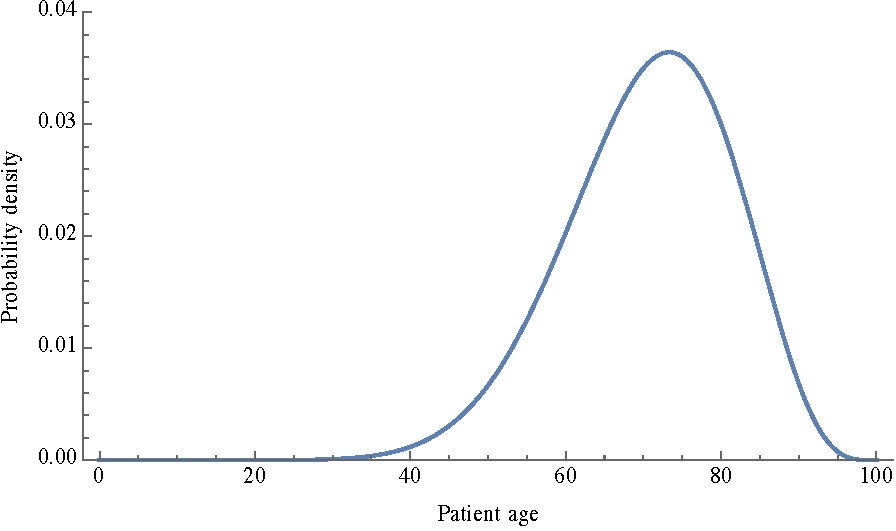
\includegraphics[scale=0.7]{hip_replacement.pdf}
    \caption{Conceptual variation of hip replacement surgeries and age}
    \label{fig:hip_replacement}
\end{figure}

With sufficient data from a given hospital, it is possible to find an age distribution function $f_i\left(a\right)$\footnote{This can be achieved by taking a sample of 1000 patients with condition $i$ or expecting treatment $i$ and examine their age distribution.} for every single component considered by one of the three mortality measures, with $a$ being the age. These three mortality measures are now represented by a finite set of functions $\left\{f_i\right\}$. Take PSIs for an example, and suppose that the target age range is between $m$ to $M$ (note that $m$ < $M$, and $0 \le m, M \le 100$). The total probability density $D_P$ from the 26 PSIs can be defined as 
\begin{gather}D_P = \sum_{i=1}^{26}\left(W_i\int_m^M \! f_i\left(a\right)\, \mathrm{d}a\right).\end{gather}

It follows that the age-adjusted component weight for a condition with index $c$ ($1 \le c \le 26$ and $c \in \mathbb{N}$) within the PSIs is 
\begin{gather}W_c\left(m, M\right) = \frac{\displaystyle W_c \int_m^M \! f_c\left(a\right)\,\mathrm{d}a}{D_P}.\end{gather}

A similar method can be used to determine the modified component weights for each of the IQIs and 30-day risk-standardized mortality measures for the given age range $m\dots M$. Once this is done, we can use the same approach as in \hyperref[sec:mortality_measures]{Section \ref*{sec:mortality_measures}} to find $R_j$, $P_j$ and $I_j$ as the three final mortality measurements, or scores, for each hospital $j$.

\subsection{Mortality and Biological Sex}

Apart from age, a couple of factors should also be accounted for when comparing hospitals through mortality measures. Biological sex is an obvious one because some conditions and their treatments are more prevalent for males or females. For instance, prostatitis\footnote{Inflammation of the prostate} is only applicable males and cervicitis\footnote{Inflammation of the cervix} is only applicable to females. In these cases, the component weight of the condition will be different for the two sexes. In fact, one will be 100\% on males and the other will have 100\% weight on females. Seeing the relevance of biological sex in mortality, it is important to add it as part of our model for mortality.

With data collected for each of the three mortality measures in \hyperref[sec:mortality_measures]{Section \ref*{sec:mortality_measures}} which we continuously refer to, we can find the gender distribution of each of the conditions. Some, of course, will be more evenly distributed than others. Then, this data can be used to construct a set of discrete functions $g_i: \left\{0,1\right\} \to [0,1]$ for every component indicator $i$ in all three mortality measures, where the input $\phi \in \{0, 1\}$ is either male $(0)$ or female $(1)$ and the output is the proportion of condition $i$ relevant to that sex. This will give new definitions (in fact, functions) for the weights. For instance, the modified weight function $W_R$ for 30-day mortality measures would be
\begin{gather}W_R\left(c, m, M, \phi\right) = \frac{\displaystyle g_c \left(\phi\right) \cdot W_c\int_m^M \! f_c\left(a\right)\mathrm{d}a}{\displaystyle\sum_{i=1}^{4}\left(g_i\left(\phi\right) \cdot W_i \int_m^M \! f_i\left(a\right) \mathrm{d}a \right)}.\end{gather}
Note that $W_R\left(c, m,M,\phi\right)$ is a valid weighting scheme for 30-day risk-standardized mortality measures (which can be generalized to the two other mortality aspects as well) because $$m, M \in \left[0,100\right], \phi \in \{0,1\} \implies \sum_{i=1}^4 W_R\left(i, m,M,\phi\right) = 1.$$
Therefore,
\begin{gather}R_j = \sum_{i=1}^4 W_R \left(i, m,M,\phi\right) \frac{\text{\# of deaths due to condition $i$ at hospital $j$}}{\text{\# of total discharged patients of treatment $i$ at hospital $j$}} \end{gather}

Similarly, we replace $W_i$ for both PSIs and IQIs with $W_P\left(i,m,M,\phi\right)$ and $W_I\left(i,m,M,\phi\right)$ respectively for each condition or treatment $i$ and use these modified weights for the final evaluation of $P_j$ and $I_j$ for each hospital $j$.

\subsection{Accuracy of Primary Diagnosis}

Due to the vast number of possible areas to explore for mortality measures, we cannot cover all of them within the length of this paper. We will consider one last factor for mortality --- the accuracy of primary diagnosis. Intuitively, it is very important to choose hospitals which do not accidentally diagnose positive cases as negative or vice versa, since some conditions have diagnosable signs that would lead to the exacerbation of the patient's health (could even lead to death) if not diagnosed and treated in time. Previously, we only evaluated the mortality of a hospital based on patients that it treats, but what if the hospital fails to diagnose the conditions of many patients with life-threatening health problems? Surely, a fourth aspect of mortality is needed to fully evaluate the quality of a hospital.

A widely recognized representation of a hospital's diagnosis accuracy is the receiver operating characteristic (ROC) curve, which shows a \textbf{trade-off} between the likelihood of correct diagnosis for patients with actual health conditions and the likelihood of wrong diagnosis for patients who don't actually have a health condition. To construct this hospital-specific curve, four quantities need to be collected from its data, namely the number of true positive (TP) assessments, true negative (TN) assessments, false positive (FP) assessments and false negative (FN) assessments, as defined in \hyperref[tab:diagnosis_matrix]{Table \ref*{tab:diagnosis_matrix}}.

{\renewcommand{\arraystretch}{1.8}%
\begin{table}[htbp]
    \centering
    \begin{tabular}{l|l|l}
        \toprule
        \multirow{ 2}{*}{Result of Diagnosis} & \multicolumn{2}{c}{Actual Patient's Condition} \\
        \cline{2-3}
        & Positive & Negative \\
        \hline
        Positive & True Positive & False Positive \\
        \hline
        Negative & False Negative & True Negative \\
        \bottomrule
    \end{tabular}
    \caption{2$\times$2 matrix definition of four diagnosis outcomes in diagnosis accuracy evaluation}
    \label{tab:diagnosis_matrix}
\end{table}
}

We define
\begin{align}
\textbf{Accuracy} = &\ \frac{\text{TP} + \text{TN}}{\text{TP} + \text{TN} + \text{FP} + \text{FN}}
\end{align}
Since wrong treatments that do not match patients' physical conditions can inflict additional health problems on them, \textbf{accuracy} is a mortality measure that indicates the probability that the diagnosis of a hospital will lead to positive outcomes for the patient regarding their health. The four variables, which sum up to the total number of diagnoses that took place in a fixed time period, are related and shown on a typical ROC curve as in \hyperref[fig:roc]{Figure \ref*{fig:roc}}.

\begin{figure}[htbp]
    \centering
    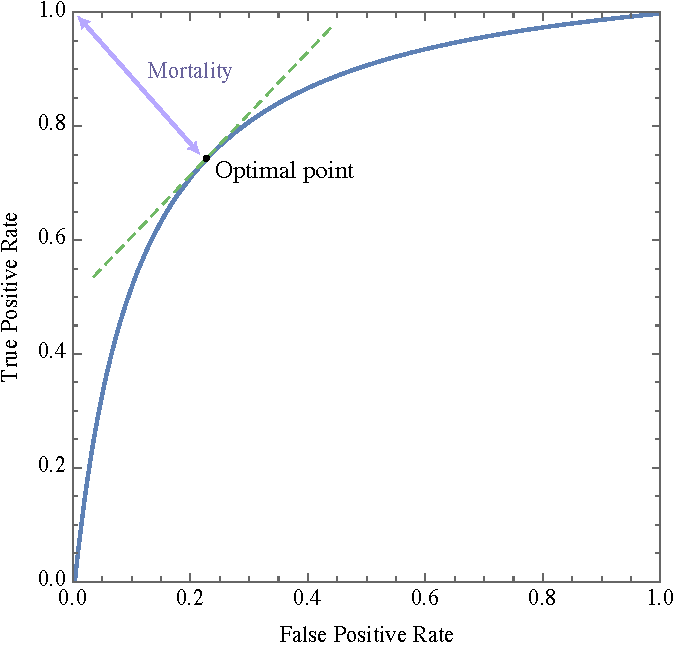
\includegraphics[scale=.78]{ROC.pdf}
    \caption{Receiver Operating Characteristic Curve for a hospital's diagnosis ability}
    \label{fig:roc}
\end{figure}

The shape of the ROC curve for each hospital $j$, described by some function $r_j : [0,1] \to [0,1]$, allows a comparison between hospitals in terms of their diagnostic accuracy. The points $[0,0]$ and $[1,1]$ must be intersected by all ROC curves, and represent the most insensitive and sensitive diagnoses respectively. At $[0,0]$, a hospital could diagnose everyone as negative, which obviously prevents healthy patients from accidentally diagnosed as positive and receiving treatments that they should not receive; at $[1,1]$, a hospital diagnoses everyone as positive regardless of their true physical conditions, which minimizes the chance of overlooking any patient with actual need of treatment. Ideally, all hospitals, regardless of their facilities and faculty skills, would want to operate at the unique point where $r_j'(x) = 1$. This is because the trade-off between ``lenience" and ``stringency" is kept minimum. At any $x$ where $r_j'(x)$ > 1, the hospital tends to increase its \textbf{true positive rate} by being more stringent with its diagnosis, knowing that this increase comes with a relatively smaller cost (i.e.\ a less-than-proportional increase in \textbf{false positive rate}). On the other hand, if a hospital is currently at a point $x$ where $r_j'(x) < 1$, then it should decrease its \textbf{false positive rate}, knowing that it comes at a smaller cost (i.e.\ a less-than-proportional decrease in \text{true positive rate}). Therefore, this optimal point is also where the diagnostic accuracy is maximized, and likely to be the place that the hospital operates in the long-run (due to the inverse relationship between \textbf{false positive rate} and \textbf{true negative rate}). 100 multiplied by the maximum diagnostic accuracy (in order to give a score out of 100) can then be calculated for each hospital and used as one of the measures for mortality, assuming that both wrong treatment and lack of treatment when needed could lead to evitable deaths. For clarification, it means that now our model for mortality now consists of four aspects for each hospital $j$, namely $R_j$, $P_j$, $I_j$ and $A_j$. We believe that these factors should not be merged into one single number for cross-comparison, since different patients may value each indicator differently. Moreover, $R_j$, $P_j$, and $I_j$ vary depending on the patient's age and gender.

To organize this information into a form that eases comparison with other quality indicators that will be introduced in the next section, we let \textbf{Q0} be a matrix with $k$ rows and $c$ columns, where $k$ is the number of hospitals, and $c$ is the total number of specialties considered. Each individual value $\mathbf{Q0}_{ji}$ would be the return value of a function $V_j\left(i,R_j, P_j, I_j, A_j\right)$ that gives a final mortality score for specialty $i$ at hospital $j$ by first finding the mean of the values $(100-R_j)$, $(100-P_j)$, $(100-I_j)$, $A_j$ that apply, and then mapping the mean to the closed interval $[0,100]$ through an exponential function. For instance, if we want to give a mortality score for a particular hospital $j$ based on $i$ = hip replacement, then $P_j$, $I_j$ and $A_j$ are applicable, and
\begin{gather}\label{eq:mortality_eval}
    V_j\left(i, P_j, I_j, A_j\right) = 100\exp\left[\frac{(100-P_j) + (100-I_j) + A_j}{3} - 100\right] - \left(100 - \frac{(100-P_j) + (100-I_j) + A_j}{3}\right) e^{-100}
\end{gather}

Note that the best mortality score a hospital can get is 100 if it has 0 deaths from all of the three mortality measures (in table \ref{sec:mortality_measures} and 100 accuracy. On the other hand, 100\% death rates for all of the three mortality measures and 0 accuracy would give a mortality score of 0, the worst possible. (We assume that accuracy $A_j$ for each hospital $j$ is independent from the specialty)

Based on \hyperref[eq:mortality_eval]{Equation \ref*{eq:mortality_eval}}, we can construct a $k \times c$ quality matrix $\mathbf{Q0} = \textit{q0}_{ji}$ representing the standardized (0 - 100) mortality score of every hospital $j$ based on each specialty $i$. If a specialty is unavailable at a hospital, we assign that spot in the matrix with 0 mortality score.

\section{Beyond Mortality}
Surely, not everybody seeks for health care at hospitals because they are facing immediate life-threatening physical conditions. Most of the times, we just need to get treated for minor illnesses. Therefore, mortality itself is not a holistic evaluation of the quality of a hospital. Besides mortality, there are also many other factors, such as the quality of the medical facilities and services, the availability of doctors, pricing, location, or the amount of training people received, each corresponding to some weighting out of 100\%. Let $n$ be the total number of factors (quality indicators) considered, and let $q_{ji}$ be a quality score for specialty $i$ at hospital $j$, which can be organized into a 2-D \textbf{quality matrix} $\mathbf{Q}$ with $i$ rows and $j$ columns. To distinguish between indicators, we use $\mathbf{Q1}$, $\mathbf{Q2}$, $\dots$, $\mathbf{Qn}$ to denote the quality matrix for each of the $n$ quality indicators considered, which are organized into a vector $\mathcal{Q}$. When given a specialty $i$, this arrangement allows us to directly compare hospitals 1 through $k$ by referring to their specialty-specific ranking score $h_{ji}$ based on the $k \times c$ \textbf{hospital comparison matrix}:
\begin{gather}\label{eq:hospital_comparison}
    \textbf{H} = (h_{ji}) =
    \begin{pmatrix}
    \sum_{z=1}^{n} (\mathcal{Q}_z)_{11} W_z & \cdots & \sum_{z=1}^{n} (\mathcal{Q}_z)_{1c}W_z \\
    \vdots & & \vdots \\
    \sum_{z=1}^{n} (\mathcal{Q}_z)_{k1}W_z & \cdots & \sum_{z=1}^{n} (\mathcal{Q}_z)_{kc} W_z
    \end{pmatrix}
\end{gather}
where $W_z$ is the weighting for the $z$-th quality indicator.

To make sure that the indicators are standardized and equitable, we adjust each individual quality value $q_{ji}$ to be a score from 0 - 100 through a mapping function $V : \mathbb{R} \to [0,100]$, where $\mathbb{R}$ could be any unit, from time units to percentages. In the rest of this section, we will discuss several important quality indicators that our model will consider.

\subsection{Success Rate of Treatment}
Perhaps what patients care most when they select a hospital is whether it can successfully treat their conditions. Typically, patients are asked to do a recheck a few days or a few weeks after their initial treatment, so that the hospital knows whether the patient has been successfully treated. Since all hospitals prefer to have 100\% success rate, it is likely that they do not publish records where patients have not been successfully treated. Nevertheless, our model assumes that the data provided by hospitals are authentic and correctly reflect their true treatment abilities. Suppose that there are $c$ physical conditions in the world, each of which hospital $j$ can treat with success rate $r_c$. We can sort these rates into a $c$-dimensional column vector $\mathbf{S}_j$. Combining the vectors from all $k$ hospitals, we have \textbf{S}, a matrix with $k$ rows and $c$ columns that comprises the success rate for each specialty for each hospital, as follows.
\begin{gather}
    \textbf{S} = 
    \begin{pmatrix}
    r_{11} & r_{12} & \cdots & r_{1c}\\
    r_{12} & r_{22} & \cdots & r_{2c}\\
    \vdots & \vdots & & \vdots\\
    r_{k1} & r_{k2} & \cdots & r_{kc}
    \end{pmatrix}
\end{gather}
Note that if a particular success rate is not applicable, we assign it to 0. Assuming that the desirability of a hospital varies exponentially with its success rate, the success score evaluation function $V_{su}$ can be defined as
\begin{gather}
    V_{su}\left(r\right) = 100 e^{r-100} - (100-r)e^{-100}
\end{gather}
where $r$ is the percentage of patients who received an effective treatment for condition $i$ out of $1\dots c$ from the $j$-th hospital out of $1 \dots k$. This can be considered as a reasonable approximation of the quality of a hospital based on its success rate, since $V_{su}\left(0\right) = 0$ and $V_{su}\left(100\right)$ = 100. Please see a visual illustration in \hyperref[fig:success_rate]{Figure \ref*{fig:success_rate}}.

\begin{figure}[htbp]
    \centering
    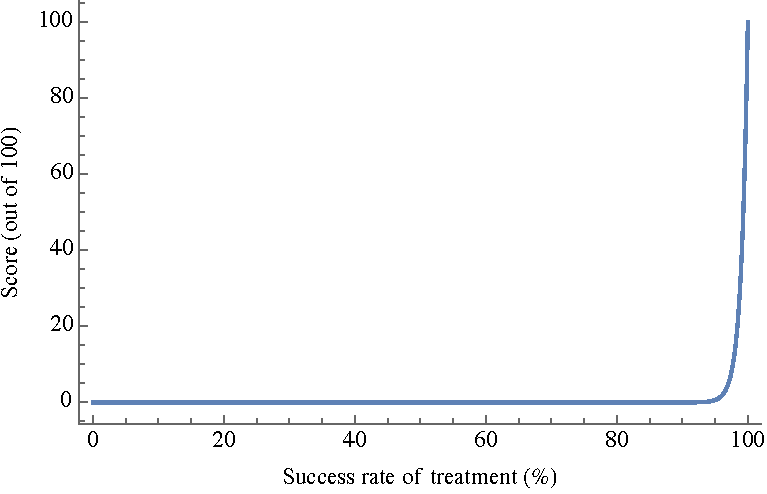
\includegraphics[scale=0.78]{success_rate.pdf}
    \caption{Relationship of success rate and success score.}
    \label{fig:success_rate}
\end{figure}

We define the standardized success score matrix $\mathbf{Q1}$ as
\begin{gather}
    \mathbf{Q1} = V_{su}\left(\mathbf{S}\right) = 
    \begin{pmatrix}
    V_{su}\left(r_{11}\right) & V_{su}\left(r_{12}\right) & \cdots & V_{su}\left(r_{1c}\right)\\
    V_{su}\left(r_{12}\right) & V_{su}\left(r_{22}\right) & \cdots & V_{su}\left(r_{2c}\right)\\
    \vdots & \vdots & & \vdots\\
    V_{su}\left(r_{k1}\right) & V_{su}\left(r_{k2}\right) & \cdots & V_{su}\left(r_{kc}\right)
    \end{pmatrix}
\end{gather}
which will later be used as part of the evaluative and comparative process for hospital ranking and selection.

\subsection{Service Quality}
Perhaps the second most important non-mortality factor that must be considered when deciding whether to go to a particular hospital is the service quality, or whether the diagnostic and treatment experience is satisfactory, from the attitudes of the faculty to indoor cleanness. Since service quality itself is a qualitative measure, we instead look at the complaints that a hospital receive. In particular, we will use the percentage of both inpatients and outpatients that fire complaints to rate each hospital ($j$), and sort this information by the hospital's specialty ($i$). The complaint rate for each hospital and specialty can be arranged into a matrix $\mathbf{C} = (p_{ji})$. For the standardized service score out of 100, we decide to use a negative exponential function, since each 1\% increase in complaints should lead to much more than 1\% of reduction in the hospital's service quality. Without question, when the quantity of complaints is 100\% for a particular specialty, the hospital scores 0 for it, and if the quantity of complaints is 0\% for the same specialty, the hospital scores 100 for it. If a specialty is unavailable, we assign the service quality to be 0.

To give the service score, we propose the following evaluation function:
\begin{gather}
    V_{se}\left(p\right) = 100e^{-x} - xe^{-100}
\end{gather}
where $p$ is the percentage of complaints from 0 to 100. An illustration of evaluation function $V_{se}$ is shown in \hyperref[fig:service_plot]{Figure 11}. This function matches the constraints $V_{se}\left(0\right) = 100$ and $V_{se}\left(100\right) = 0.$ We now have an expression for $\mathbf{Q2}$:
\begin{gather}
    \mathbf{Q2} = V_{se}\left(\mathbf{C}\right) =
    \begin{pmatrix}
    V_{se}\left(p_{11}\right) & V_{se}\left(p_{12}\right) & \cdots & V_{se}\left(p_{1c}\right)\\
    V_{se}\left(p_{12}\right) & V_{se}\left(p_{22}\right) & \cdots & V_{se}\left(p_{2c}\right)\\
    \vdots & \vdots & & \vdots\\
    V_{se}\left(p_{k1}\right) & V_{se}\left(p_{k2}\right) & \cdots & V_{se}\left(p_{kc}\right)
    \end{pmatrix}
\end{gather}

\begin{figure}[htbp]
    \centering
    \begin{minipage}[t]{0.5\textwidth}
        \centering
        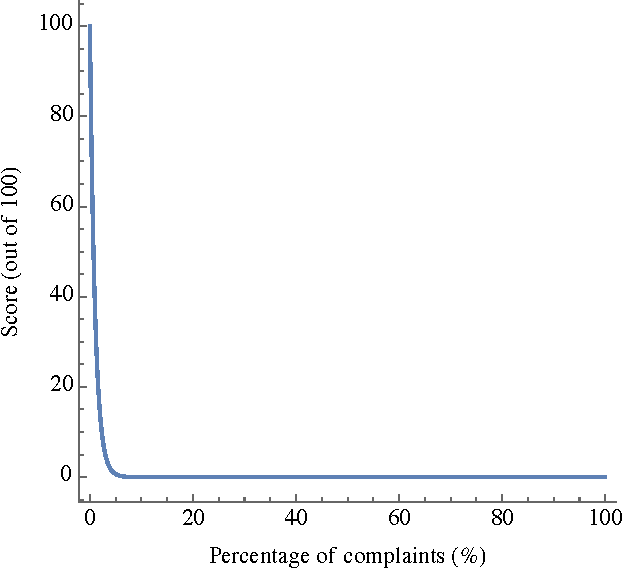
\includegraphics[scale=0.69]{service_plot.pdf}
    \end{minipage}
    \begin{minipage}[t]{0.4\textwidth}
        \centering
        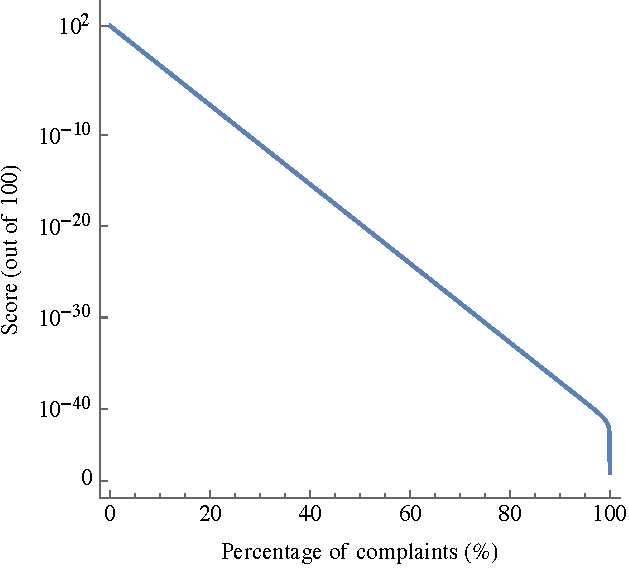
\includegraphics[scale=0.69]{log_service_plot.pdf}
    \end{minipage}
    \caption{Normal and logarithmic plot for $V_{se}\left(p\right).$}
    \label{fig:service_plot}
\end{figure}


\subsection{Availability}
Most people would want to have their illness treated as soon as possible at a hospital so they can regain a better health sooner. This would make hospitals that have better availability an optimal choice. The waiting time of a person at a hospital can be understood as the sum of all the time he is enqueue until he leaves the hospital, or the difference between the time he takes if he enters an idle hospital and the time if he enters a fully occupied hospital.

To evaluate the user experience of a hospital in terms of its availability, it requires data collected from patients in a month or year for each specialty (availability may vary across specialties). This data can be graphed into a waiting time density function $P_w\left(t\right)$, where $t$ is the total waiting time in minutes and is non-negative. Note that 
$$\int_0^\infty P_w\left(t\right) \mathrm{d}t \le 1$$
because this quantity represents the proportion of patients who need to wait at some point during their hospital visit, but it is possible that some patients have 0 waiting time (e.g. when the hospital is idle). \hyperref[fig:waiting_time_dist]{Figure \ref*{fig:waiting_time_dist}} illustrates a demonstrative $P_w$ for one specialty at a hospital, where $$P_w\left(t\right) = \frac{1.1}{1.42\pi \left[1 + \left( \frac{t -3}{1.42}\right)^2\right]}$$

\begin{figure}[!htbp]
    \centering
    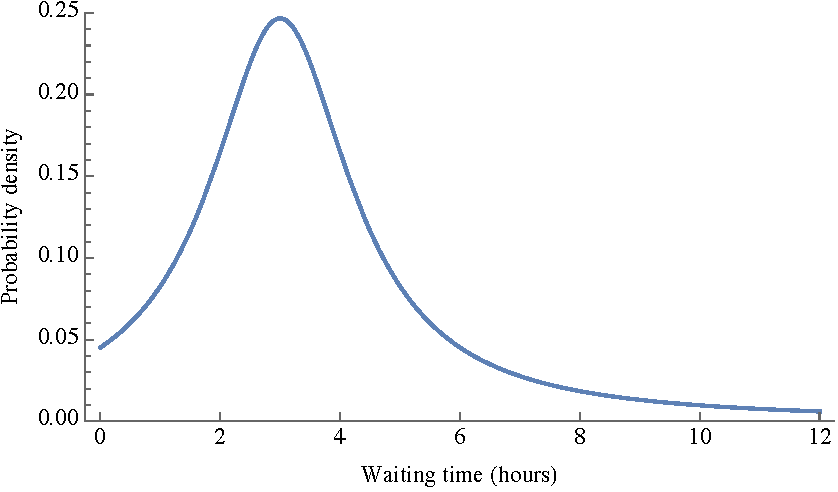
\includegraphics[scale=0.68]{waiting_time_dist.pdf}
    \caption{Waiting time distribution function for a typical hospital}
    \label{fig:waiting_time_dist}
\end{figure}

A common practice among hospitals in measuring patients' waiting time is by taking the median. For a continuous probability density function, the median is calculated by integrating the function from $-\infty$ and find the upper integration limit on the $x$-axis where the area equals to 0.5. However, this method is not directly applicable to $P_w$ in general because it is likely that the total area under the curve is less than one. To find the median, we instead integrate backward and find the median $m$ such that
\begin{gather}
    \int_m^{\infty}P_w\left(t\right) \mathrm{d}t =  \int_m^{\infty} \frac{1.1}{1.42\pi \left[1 + \left( \frac{t -3}{1.42}\right)^2\right]} = 0.5.
\end{gather}
Using technology, it is possible to find the numerical value for $m$. In this particular function, $m = 3.2042$, the median waiting time at this hospital. This is shown in \hyperref[fig:waiting_time_int]{Figure \ref{fig:waiting_time_int}}. If the entire area under the curve $< 0.5$, the median waiting time is simply 0.

\begin{figure}[!htbp]
    \centering
    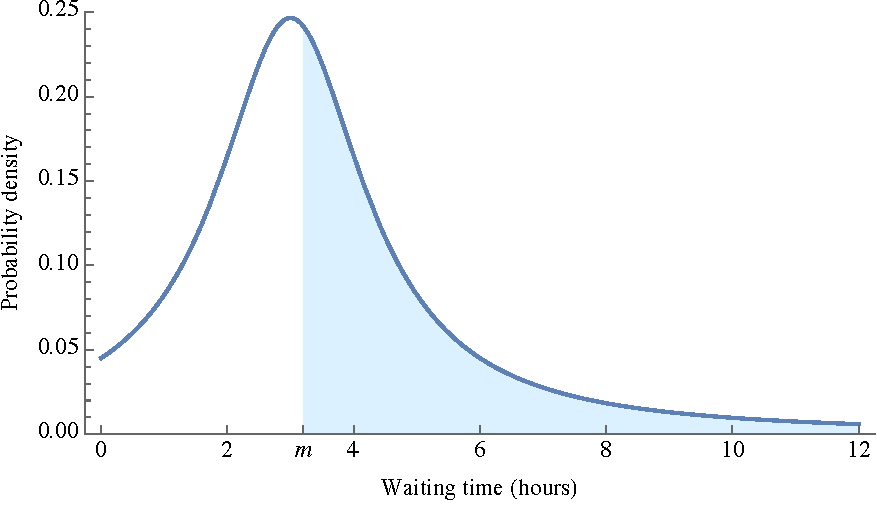
\includegraphics[scale=0.7]{waiting_time_int.pdf}
    \caption{Backward integration method to find the median waiting time for a hospital}
    \label{fig:waiting_time_int}
\end{figure}

In a particular city or country, there are $k \times c$ number of these waiting time density functions, since each of the $k$ hospital has a $P_w$ curve for each of its $c$ specialties, (N/A if no such department exists for a given specialty, but it still counts). We can arrange the median waiting time for all specialties and hospitals into a matrix $\mathbf{T} = (m_{ji})$.

As previously stated, the raw value for each indicator must be converted to some function that gives a score out of 100. From our survey results, the vast majority of people's maximum tolerance of waiting time is 5 hours. This value will be the ``cut-off" point in the sense that any hospital with median waiting time of 5 hours or higher gets 0 point for this quality indicator, and a hospital with 0 median waiting time earns 100 points. In addition, if $t$ = N/A, the score is 0. With these criteria met, we define the following evaluation function for hospital waiting time
\begin{gather}
V_w\left(t\right) =
\begin{dcases}
    100e^{-t} + \frac{t}{20}e^{-5} & 0 < t < 5\\
    0 & t \ge 5 \text{ or } t = \text{N/A}.
\end{dcases}
\end{gather}
where $t$ is the median waiting time as previously defined. This yields the quality matrix $\mathbf{Q3}$, defined as follows:
\begin{gather}
    \mathbf{Q3} = V_w\left(\mathbf{T}\right) =
    \begin{pmatrix}
    V_w\left(m_{11}\right) & V_w\left(m_{12}\right) & \cdots & V_w\left(m_{1c}\right)\\
    V_w\left(m_{12}\right) & V_w\left(m_{22}\right) & \cdots & V_w\left(m_{2c}\right)\\
    \vdots & \vdots & & \vdots\\
    V_w\left(m_{k1}\right) & V_w\left(m_{k2}\right) & \cdots & V_w\left(m_{kc}\right)
    \end{pmatrix}
\end{gather}
A graph for $V_w$ is shown in \MRef{Figure}{fig:v_w}.

\begin{figure}[htbp]
    \centering
    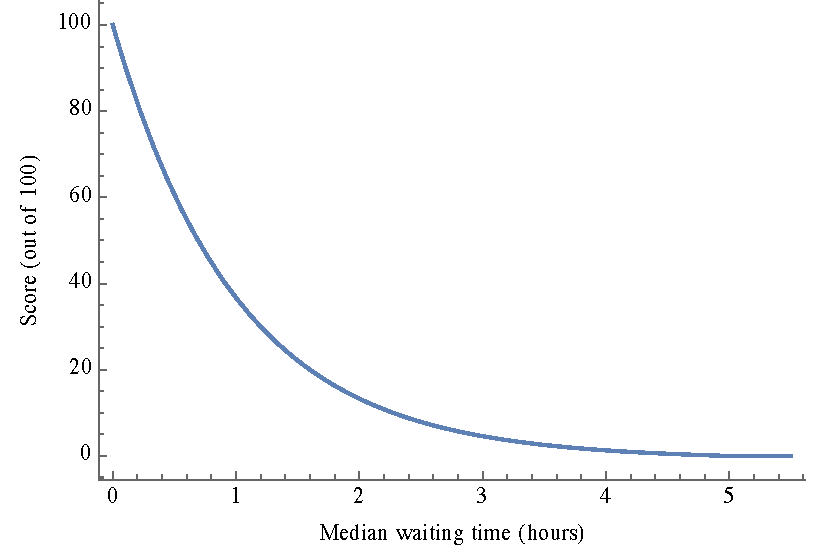
\includegraphics[scale=0.75]{V_w.pdf}
    \caption{Variation of availability score for a hospital with its median waiting time}
    \label{fig:v_w}
\end{figure}

Note that the shape of the curve is concave upward due to the fact that patients generally tend to lose their satisfaction at a rate faster than proportional to their waiting time.

\subsection{Performance on Controlling Epidemics}

A quality indicator that people often ignore is whether a hospital is efficient at controlling an epedemic, which may be an important factor when judging the contribution that a hospital makes in combating a city- or nation-wide disease like the influenza. Nowadays, epidemics are generally covered in the national health care programs of the United Kingdom and the Republic of France and are common worldwide. Thus, the performance of hospitals in controlling the spread of such diseases is another crucial criterion in evaluating the integral quality of the treatments by those hospitals. Various differential dynamical systems have been developed to interpolate and predict the growth of different types of epidemics among a sample population.

We will now examine a modified version of the \textbf{Susceptible-Infected-Recovered (S-I-R) model} without vital dynamics (The Medical S.I.R. Equations) estimating the change of susceptible, infected, and recovered population with respect to time in an isolated and static region, (i.e. to ignore the natural birth and death of the population and the emigration and immigration), and with intervention of a specific hospital.

In the Medical S.I.R. model, we need to assume the that the recovered population $N \ge 0$ has permanent immunity to the epidemic. Functions $S(t),I(t),R(t)\in\mathbb{R}\to\mathbb{R}_{\geq0}$ respectively denote the population of susceptible, infected, and recovered population at a specific time $t$. Moreover, parameters $\beta\geq0$ is the spread-efficiency coefficient, $\gamma\geq0$ is the immune system's self-healing-efficiency coefficient, $\mu\geq0$ is the efficiency of the institution's immunization program, and $\nu\geq0$ is the efficiency of the institution's treatment. the relation between the instantaneous rates of changes of the susceptible, infected, and recovered population can be described by the differential dynamical system shown by (\ref{eqn:sir}).

\begin{gather}
\label{eqn:sir}
\begin{dcases}
\frac{dS}{dt}=-\frac{\beta}{N}IS-\mu S\\
\frac{dI}{dt}=\frac{\beta}{N}IS-\gamma I-\nu I\\
\frac{dR}{dt}=\gamma I+\mu S+\nu I
\end{dcases}
\end{gather}

The generic analytic solution functions of the classical S.I.R. model has not yet been found, thus we shall not pursue such solution.  Rather, we focus on the qualitative properties of the dynamical system. Based on the assumption that all parameters and the values of functions $S(t),I(t),R(t)$ are non-negative, we are able to conclude the monotonicity of $S(t)$ and $R(t)$ for all $t$. For the function $I(t)$, we are able to find one $t_0$ such that $I'(t_0)=0$, which is at a $t_0$ such that \[S(t_0)=\frac{N}{\beta}\left(\gamma+\frac{\nu}{I(t_0)}\right).\]

Now one might invoke the classical S.I.R. model (\ref{eqn:sir_org}) for comparison, where the maximum of $S(t)$ is still unique but at a $t_0$ such that \[S(t_0)=\frac{N}{\beta}r.\]

\begin{gather}
\label{eqn:sir_org}
\begin{dcases}
\frac{dS}{dt}=-\frac{\beta}{N}IS\\
\frac{dI}{dt}=\frac{\beta}{N}IS-\gamma I\\
\frac{dR}{dt}=\gamma I
\end{dcases}
\end{gather}

To provide an demonstration of the maximum behaviour of both two model, we employ the numerical method to plot a time-versus-population graph of the dynamical systems with some \textbf{demonstrative parameters}(\MRef{Table}{tab:demo_parameters_ori_sir}).

\begin{table}[htbp]
        \centering
        \caption{Demonstrative Arbitrary Parameters for S.I.R.}\\[4pt]
        \label{tab:demo_parameters_ori_sir}
        \begin{tabular}{c|c|c}
            Parameter & Implication & Value \\\hline
            $\beta$ & Infection spreading efficiency & 2 \\
            $\gamma$ & Human immune system self-curing efficiency & .1 \\
            $N$ & Total population & 1000 \\\hline
            $S(0)$ & Initial susceptible population & 999 \\
            $I(0)$ & Initial infected population & 1 \\
            $R(0)$ & Initial recovered population & 0 \\\hline
            $\epsilon$ & $\sup\mathrm{err}$ & .1 \\
            $c$ & $\sup\Delta t$ & .1 \\
            $N$ & Step limit & 500 \\
        \end{tabular}
        \end{table}

The graph generated by an adaptive Euler's approximation method of the classical S.I.R. model is shown in \MRef{Figure}{fig:euler_ori_sir}.

\begin{figure}[htbp]
\centering
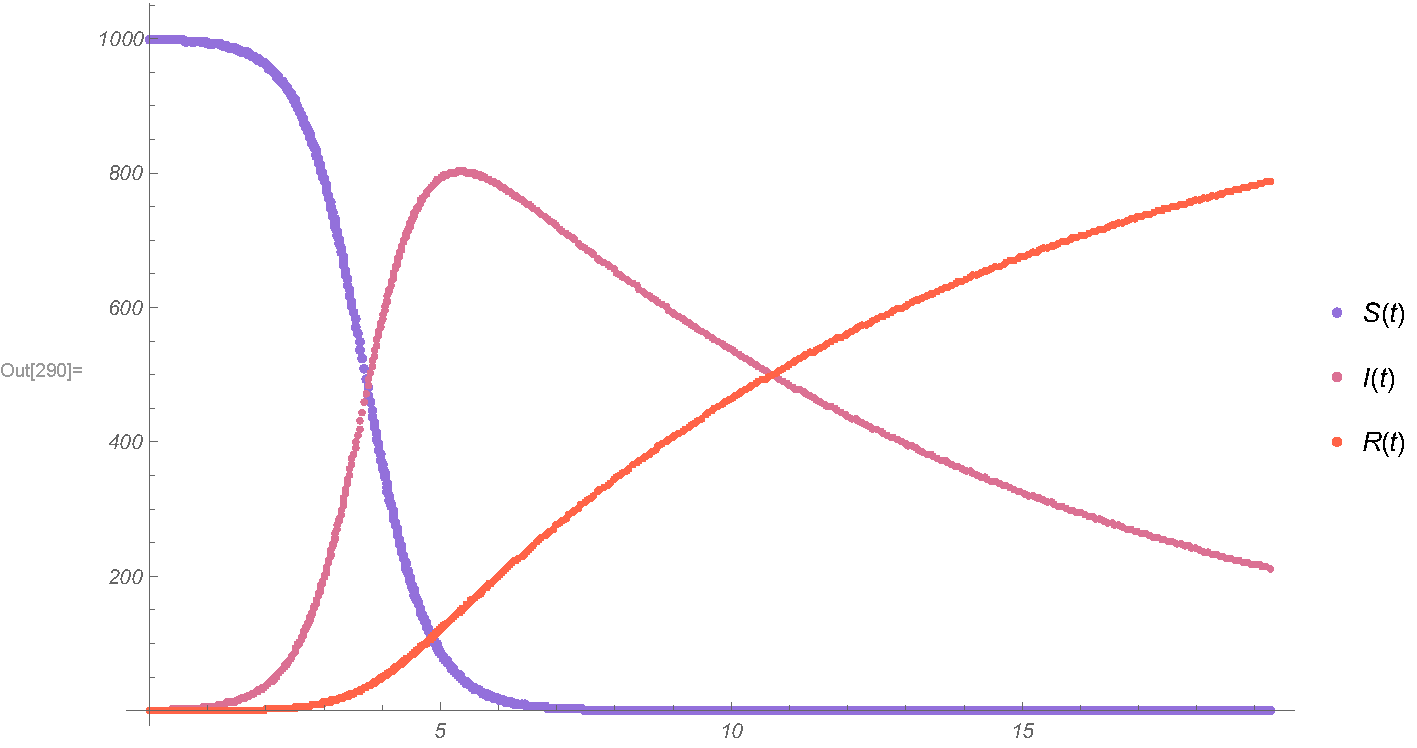
\includegraphics[scale=.45, clip, trim=37.5pt 0 0 0]{AdaptiveEulerOriginalSIR.pdf}
        \caption{Plot of the Euler approximation of functions $S(t), I(t), R(t)$ in the classical S.I.R. model (\ref{eqn:sir_org}) with demonstrative parameters (\MRef{Table}{tab:demo_parameters_ori_sir})}
        \label{fig:euler_ori_sir}
\end{figure}
\newpage
Then, for comparison, we also use a set of demonstrative data to elaborate the intervention of a medical institution, as shown in  \hyperref[tab:demo_parameters_mod_sir]{Table \ref*{tab:demo_parameters_mod_sir}} and \hyperref[fig:euler_mod_sir]{Figure \ref*{fig:euler_mod_sir}}.

\begin{table}[htbp]
    \centering
    \caption{Demonstrative Arbitrary Parameters for Modified S.I.R.}\\[4pt]
    \label{tab:demo_parameters_mod_sir}
    \begin{tabular}{c|c|c}
         Parameter & Implication & Value \\\hline
         $\beta$ & Infection spreading efficiency & 2 \\
         $\gamma$ & Human immune system self-curing efficiency & .1 \\
         $N$ & Total population & 1000 \\\hline
         $\mu$ & Hospital's immunization program's efficiency & .1 \\
         $\nu$ & Hospital's treatment (for infected subjects)'s efficiency & .1 \\\hline
         $S(0)$ & Initial susceptible population & 999 \\
         $I(0)$ & Initial infected population & 1 \\
         $R(0)$ & Initial recovered population & 0 \\\hline
         $\epsilon$ & $\sup\mathrm{err}$ & .1 \\
         $c$ & $\sup\Delta t$ & .1 \\
         $N$ & Step limit & 500 \\
    \end{tabular}
\end{table}

\begin{figure}[htbp]
    \centering
    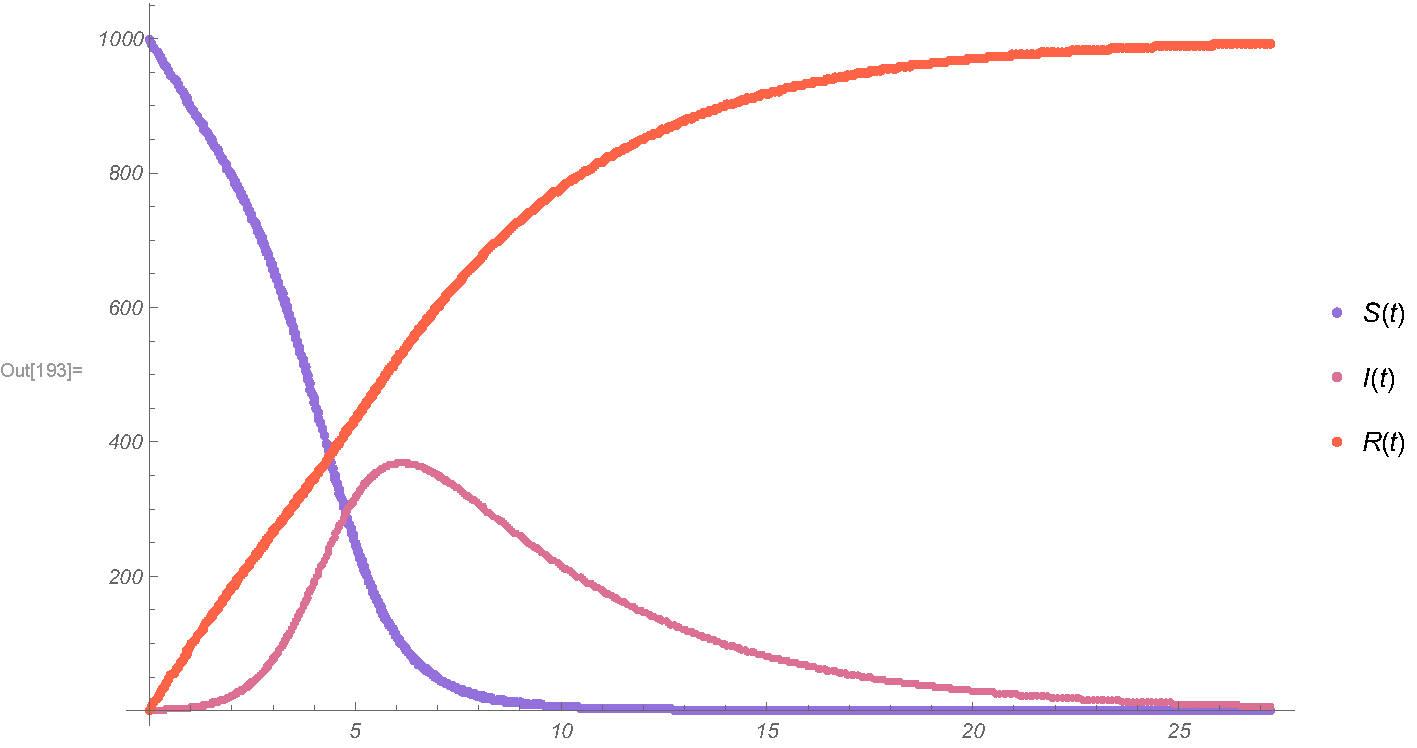
\includegraphics[scale=.45, clip, trim=37.5pt 0 0 0]{AdaptiveEulerModifiedSIR.pdf}
    \caption{Plot of the Euler approximation of functions $S(t), I(t), R(t)$ in the modified S.I.R. model (\ref{eqn:sir}) with demonstrative parameters (\MRef{Table}{tab:demo_parameters_mod_sir})}
    \label{fig:euler_mod_sir}
\end{figure}

Now, according to the numerical solution to the demonstrative functions, we have a maximum point of $I(t)$, $(t_0,I(t_0))$, at \begin{gather}\label{eqn:max_i_classical_sir}(5.34503, 801.856)\end{gather} in the classical equations, and a $(t_0,I(t_0))$ at \begin{gather}\label{eqn:max_i_modified_sir}(6.15082, 368.417)\end{gather} in the modified S.I.R. model.

At this point we have no evident observation as to the degree of intervention on the dynamics behaviour of the epidemic disease itself, with only one definite perspective that when $t\to t_0$, where \begin{gather}\label{eqn:gen_max_i_classical_sir}S(t_0)=\frac{N}{\beta}\gamma,\end{gather} $$\displaystyle{\therefore I(t)\to\max_{t\in[0,+\infty)}I(t)}$$ in the classical S.I.R. model, and when that occurs, \begin{gather}\label{eqn:gen_max_i_modified_sir}S(t_0)=\frac{N}{\beta}\left(\gamma+\nu\right)\end{gather} in the modified S.I.R. model. In the real world, the above properties imply that when the hospital starts to make influences to the dynamical system, it has a relative large-scaled effect (as seen in the scale comparison of the total population $N$ and the parameter $\mu$ and $\nu$), and the parameter $\nu$ has a considerable impact on the position of the maximum point of $P(t)$, as seen in comparison between (\ref{eqn:max_i_classical_sir}) and (\ref{eqn:max_i_modified_sir}) (the comparison between the generic term (\ref{eqn:gen_max_i_classical_sir}) and (\ref{eqn:gen_max_i_modified_sir}) can support and further explain this phenomenon).

Presumably, from \MRef{Figure}{fig:euler_ori_sir} and \MRef{Figure}{fig:euler_mod_sir}, it is of the best interest of a hospital delay and postpone the maximum in the time axis as long as possible and to decrease the value of $I(t)$. Thus, we conclude this analysis with an evaluation function
\begin{gather}
\label{eqn:eval_func_mod_sir}
V_\iota\left(T,\mathcal{T}_,\,I,\mathcal{I}\right)= 100\left(1-\frac{1}{\mathrm{Re}\left(\sqrt{\mathcal{T}-T}\right)+1}\right)\cdot\left(\frac{\left(\sqrt{I}+\sqrt{I+4 \sqrt{I}}+2\right) \mathrm{Re}\left(\sqrt{I-\mathcal{I}}\right)}{\left(\sqrt{I}+\sqrt{I+4 \sqrt{I}}\right) \mathrm{Re}\left(\sqrt{I-\mathcal{I}}\right)+2 \sqrt{I}}\right),
\end{gather}
where $T$ and $\mathcal{T}$ denote $t_0$ at which point the function $I(t)$ reaches its sole maximum in the classical and modified S.I.R. equations respectively, and $I$ and $\mathcal{I}$ represent the value of the function when reaching the maximum for the classical and modified S.I.R. model respectively. When
\[
\begin{dcases}
T\geq0\\
\mathcal{T}\geq T\\
I>0\\
\mathcal{I}\geq I
\end{dcases},
\]
the value of the evaluation function $V_\iota\left(T,\mathcal{T}_,\,I,\mathcal{I}\right)$ is guaranteed to be within $[0,100]$, which would suffice the requirement of an evaluation function.

When $\displaystyle{I=\max_{t\in[0,+\infty)}I(t)=10}$, the behaviour of $V_\iota\left(T,\mathcal{T}_,\,I,\mathcal{I}\right)$ could be demonstrated with \ref{fig:msir_eval_func_plot}.

\begin{figure}[htbp]
    \centering
    \begin{minipage}[t]{0.5\textwidth}
        \centering
        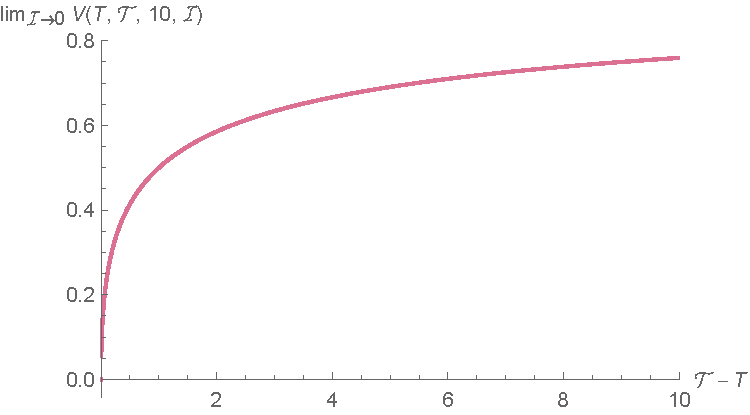
\includegraphics[width=\textwidth]{EvalFuncMSIR1.pdf} % first figure itself
    \end{minipage}\hfill
    \begin{minipage}[t]{0.5\textwidth}
        \centering
        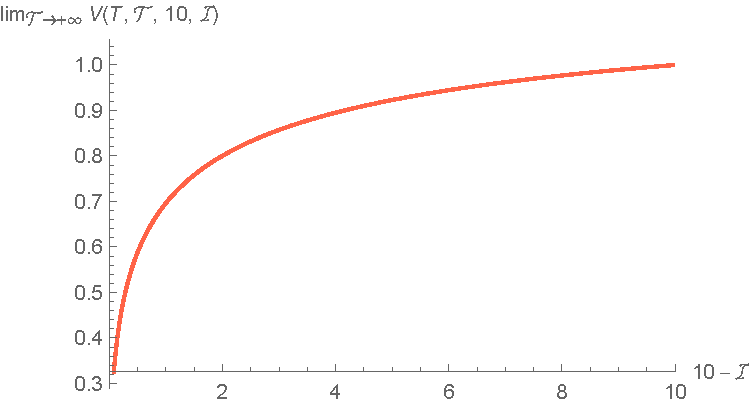
\includegraphics[width=\textwidth]{EvalFuncMSIR2.pdf} % second figure itself
    \end{minipage}
    \caption{Demonstration of 2 multipliers of the evaluation function $V_\iota\left(T,\mathcal{T}_,\,I,\mathcal{I}\right)$}
    \label{fig:msir_eval_func_plot}
\end{figure}

One example of an epidemic disease that has a stage transformation sequence as described with the classical and modified S.I.R. would be \mathbf{epidemic parotitis}, a.k.a. mumps, colloquially, and the data from the Disease Control Center of Shenyang City applied with this model along with the evaluation (using (\ref{eqn:eval_func_mod_sir})) of this facility acting as an administrative hospital would be provided in the appendix.

Using \hyperref[eqn:eval_func_mod_sir]{Equation 29}, we have
\begin{gather}
\mathbf{Q4}=
\begin{pmatrix}
V_\iota(T_{i,j},\mathcal{T}_{i,j},\,I_{i,j},\mathcal{I}_{i,j})
\end{pmatrix}_{(M\times N)}
\end{gather}

\subsection{Pricing and Location}

Considering that we live in the digital age, it is very likely that many patients use mobile apps or websites to determine the ``best" hospital to them, and generally algorithms will not only consider the quality of the hospitals themselves, but also their real-time location and the affordability of the hospitals to see whether it's worth going for a very far hospital just to get a more professional or cheaper treatment. Oftentimes, patients would place the quality of their treatments at the priority relative to the hospital's price and location, but not all the times. One theoretical exception is when two hospitals have identical rankings for the hospital qualities, and now the only discerning factors are the prices and locations of the two hospitals. Therefore, these factors should be accounted for in our model with a very small weight. More specifically, location and price must be modelled as probability distributions, since the preference of each patient may vary depending on situational factors such as the level of hurriedness. In this short section, we will only consider the location and price of each hospital and add them as part of the algorithm that helps patients to find the most suitable hospital for them. Let $\mathbf{d} = d_{j}$ be the vector that records the distance of the patient from each hospital $j$, and let $\mathbf{P} = p_{ji}$ be the vector that records the price level of each hospital by its departments for every specialty $i$.

In our team's paper for IMMC 2018 regional round, we identified a probability mass function $P\left(D, S_i, \gamma\right)$ that finds the probability that a customer at point $D$ is going to visit each of the $i$ stations $S_1\dots S_i$, given a constant $\gamma$ that we refer to as the \textbf{distance selection bias} $(= \log_{1.1}(2) \approx 7.2725)$, or how sensitive people are to distances:
\begin{gather}
    P_d\left(D, S_i, \gamma_l\right) = \lim_{m \to 0} \frac{\left[ d\left(D, S_i\right) + m \right]^{-\gamma}} {\displaystyle\sum_{k=1}^n \left[d\left(D, S_k\right) + m \right]^{-\gamma}}
\end{gather}

However, in the case of hospital selection, we can assume that the distance of every hospital to each patient is given, since it is easy to calculate them using digital software, which patients are likely to be using. Let $\{D_1\dots D_k\}$ be the set of absolute distances between the patient and each of the $1\dots k$-th hospital, then the new location-wise preference distribution can be modelled by
\begin{gather}
     P_d\left(D_i, \gamma_d\right) = \lim_{m \to 0} \frac{(D_i + m)^{-\gamma_d}}{\displaystyle\sum_{k=1}^n (D_k + m)^{-\gamma_d}}.
\end{gather}
where $\gamma_d$ is the new symbol for $\gamma$ since we need to distinguish between the distance bias $\gamma_d$ and price bias $\gamma_p$.

To determine the relative importance of price relative to distance, we have conducted a survey, and found that when the proportional difference in price and distance is identical, 57\% of respondents value price over distance. This implies that the majority of people (at least those that participated in the survey) are more responsive to price differences than location differences. As a result, we expect $\gamma_p > \gamma_d$, where $\gamma_p$ is the \textbf{price selection bias}. Let $\{\rho_1\dots\rho_k\}$ be the price levels for each of $1\dots k$ hospitals. The price-wise preference distribution can be modelled by
\begin{gather}
    P_p\left(\rho_i, \gamma_p\right) = \lim_{m \to 0} \frac{(\rho_i + m)^{-\gamma_p}}{\displaystyle\sum_{k=1}^n (\rho_k + m)^{-\gamma_p}}.
\end{gather}

We can determine the exact value of $\gamma_p$ by expressing it in terms of $\gamma_d$ using the result of the survey, which presents a scenario where hospital $A$ is close but expensive by 10\% of $B$ and $B$ is farther by 10\% comparing to $A$ but cheaper comparing to $A$. Since $P \left(\rho_i, \gamma_p\right)$ weighs 57\% and $P \left(D_i,\gamma_d \right)$ weighs 43\%, we have
\begin{align}
    43\% \times P_d \left(1.1,\gamma_d \right) + 57\% \times P_p \left(1, \gamma_p\right) & = \frac{57\%}{43\%} \left(43\% \times P_p \left(1.1,\gamma_d \right) + 57\% \times P_d \left(1, \gamma_p\right)\right) \\
   \displaystyle 43\% \lim_{m \to 0} \frac{(D_i + m)^{-\gamma_d}}{\displaystyle\sum_{k=1}^n (D_k + m)^{-\gamma_d}} + 57\% \lim_{m \to 0} \frac{(\rho_i + m)^{-\gamma_p}}{\displaystyle\sum_{k=1}^n (\rho_k + m)^{-\gamma_p}} & = 57\% \lim_{m \to 0} \frac{(D_i + m)^{-\gamma_d}}{\displaystyle\sum_{k=1}^n (D_k + m)^{-\gamma_d}} + \frac{3249}{4300} \lim_{m \to 0} \frac{(\rho_i + m)^{-\gamma_p}}{\displaystyle\sum_{k=1}^n (\rho_k + m)^{-\gamma_p}} \\
  43\% \frac{1.1^{-\log_{1.1}(2)}}{1 + 1.1^{-\log_{1.1}(2)}} + 57\%\frac{1.1^{-\gamma_p}}{1+1.1^{-\gamma_p}} & = 57\%\frac{1}{1 + 1.1^{-\log_{1.1}(2)}} + \frac{3249}{4300}\frac{1}{1 + 1.1^{-\gamma_p}}\\
  \frac{43\% + 2 \times 57\%}{3} & = \frac{\frac{3249}{4300} - 57\% \times 1.1^{-\gamma_p}}{1 + 1.1^{-\gamma_p}}\\
  157\% + 157\% \times 1.1^{-\gamma_p} & = \frac{9747}{4300} - 171\% \times 1.1^{-\gamma_p}\\
  0 & = \frac{749}{1075} - 328\% \times 1.1^{-\gamma_p}\\
  \gamma_p & = -\log_{1.1}\left(\frac{749}{1075 \times 328\%}\right)\\ & \approx 16.2541.
\end{align}

This result matches the intuitive criterion $\gamma_p > \gamma_d$ which adds to its validity.

It is not difficult to see that based on the 43:57 ratio weighting of location and price, the optimal hospital $j$ is one which the patient's distance $D_j$ and price $\rho_j$ satisfy the criterion
\begin{gather}\label{eq:max_criterion}
    43\% \times P\left(D_j, \gamma_d\right) + 57\% \times P\left(\rho_j, \gamma_p\right) = \max_{i = 1\dots k} \left[43\% \times P\left(D_i, \gamma_d\right) + 57\% \times P\left(\rho_i, \gamma_p\right)\right].
\end{gather}
For convenience, we denote $\mu_{ji} (=\!\mu_{ji}\left(\mathbf{d}, \mathbf{P}_{ji}\right))$ as the raw distance-price score for hospital $j$, $m_{dp} (=\!m_{dp}\left(\mathbf{d}, \mathbf{P}_{ji}\right))$ as the minimum possible value of $\mu_{ji}$ and $M_{dp} (=\!M_{dp}\left(\mathbf{d}, \mathbf{P}_{ji}\right))$ as the maximum possible value of $\mu_{ji}$. We can now rewrite \hyperref[eq:max_criterion]{Equation \ref*{eq:max_criterion}} in a simpler form:
\begin{gather}
    \mu_{ji} = M_{dp}.
\end{gather}
In general, we can use $\boldsymbol{\mu} = (\mu_{ji})$ as a matrix that comprises the raw distance-price score for each of the $k$ hospitals and each of the $i$ specialties within the range of consideration. If one or more values of $\boldsymbol{\mu}$ are partially unavailable due to the lack of the hospital's department for certain specialties, then we assign them as 0, since a hospital without a specialty which a patient demands should be taken out of consideration.

Next, we will consider $V_{dp}\left(\mu_{ji}\right)$, the evaluation function for distance and price that assigns a score out of 100 for each of the hospitals purely based on their location to the patient and their pricing. Obviously, two constraints of this function are:
\begin{enumerate}
    \item $V_{dp}\left(\mu_{ji}\right)$ is maximized (=100) when $\mu_{ji} = M_{dp}$;
    \item $V_{dp}\left(\mu_{ji}\right)$ is minimized (=0) when $\mu_{ji} = m_{dp}$.
\end{enumerate}

Again, like other evaluation functions, we assume that patients' preference for a hospital drops exponentially as its price and/or location increases. Therefore, a reasonable design is
\begin{align}\label{eq:dp_eval}
    V_{dp}\left(\mu_{ji}\right) & = 100e^{\mu_{ji} - M_{dp}} - \frac{M_{dp} - \mu_{ji}}{M_{dp} - m_{dp}}100e^{-m_{dp}}.\\
     \mathbf{Q5} = V_{dp}\left(\boldsymbol{\mu}\right) & =
    \begin{pmatrix}
        V_{dp}\left(\mu_{11}\right) & V_{dp}\left(\mu_{12}\right) & \cdots & V_{dp}\left(\mu_{1c}\right)\\
        V_{dp}\left(\mu_{12}\right) & V_{dp}\left(\mu_{22}\right) & \cdots & V_{dp}\left(\mu_{2c}\right)\\
        \vdots & \vdots & & \vdots\\
        V_{dp}\left(\mu_{k1}\right) & V_{dp}\left(\mu_{k2}\right) & \cdots & V_w\left(\mu_{kc}\right)
    \end{pmatrix}
\end{align}
An illustration of $V_{dp}\left(\mu\right)$ is shown in \hyperref[fig:v_dp]{Figure \ref*{fig:v_dp}}. When any number of hospitals ($k$ of them) is given, this evaluation function guarantees that at least one hospital will have a score of 100 and at least one will have a score of 0, and the rest will be in between. \hyperref[eq:dp_eval]{Equation \ref*{eq:dp_eval}} can be viewed as a composite function, since $\mu_{ji}$, $M_{dp}$ and $m_{dp}$ are all functions themselves and vary depending on $D_i$ and $\rho_i$.

\begin{figure}[htbp]
    \centering
    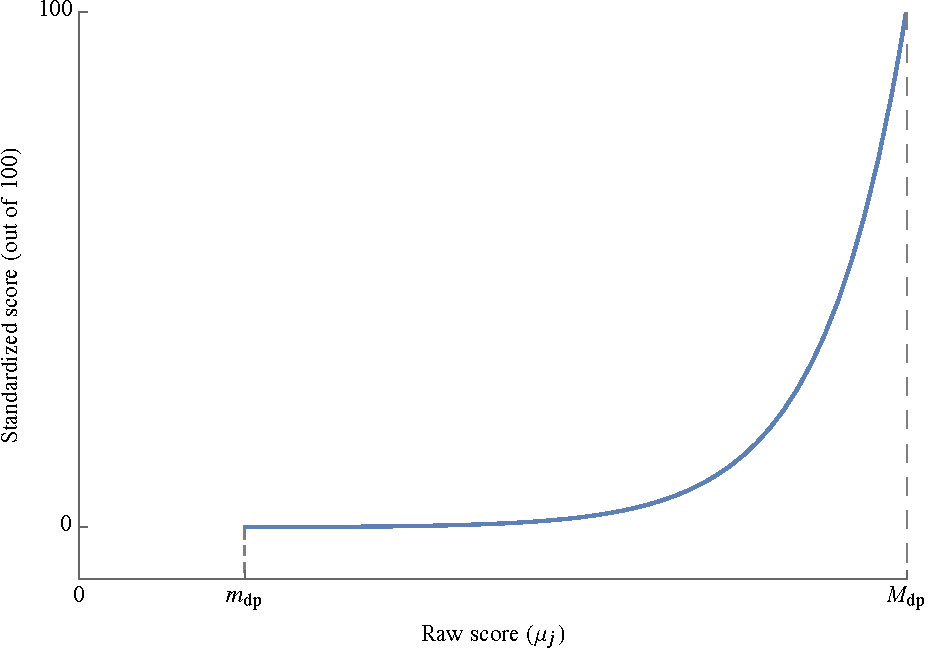
\includegraphics[scale=.72]{v_dp.pdf}
    \caption{Visualization of $V_{dp}\left(\mu_{ji}\right)$ within domain $m_{dp} \le \mu_{ji} \le M_{dp}$.}
    \label{fig:v_dp}
\end{figure}
\newpage
\subsection{All in One}

Having constructed \textbf{Q0} to \textbf{Q5}, each with $k$ rows and $c$ columns with values ranging from 0 to 100, we will need to consider the relative importance of all these factors when calculating \textbf{H}, the hospital comparison matrix, since a percentage weighting $W_i$ is needed for every one of the 6 factors. To correctly determine the weights, we conducted another survey, and obtained the a weight distribution shown in \hyperref[tab:weightings]{Table \ref*{tab:weightings}}.

{\renewcommand{\arraystretch}{1.2}%
\begin{table}[htbp]
    \centering
        \caption{Quality Indicators and Weightings from Survey Results}\\[4pt]
    \begin{tabular}{l|l}
        \textbf{Quality Indicator} & \textbf{Weighting Percentage ($W_i$)}\\
        \hline
        Mortality & 11.3\% \\
        Success rate & 19.2\% \\
        Service quality & 19.1\% \\
        Median waiting time & 15.9\% \\
        Control of epidemics & 16.4\% \\
        Location and price & 18.1\%
    \end{tabular}    \label{tab:weightings}
\end{table}}

Therefore, with definition from equation \hyperref[eq:hospital_comparison]{Equation \ref*{eq:hospital_comparison}}, we have
\begin{gather}
    \mathbf{H} = 11.3\% \times \mathbf{Q0} + 19.2\% \times \mathbf{Q1} + 19.1\% \times \mathbf{Q2} + 15.9\% \times \mathbf{Q3} + 16.4\% \times \mathbf{Q4} + 18.1\% \times \mathbf{Q5}
\end{gather}

This means that for a patient seeking for a treatment under the $i$ specialty, his/her best option is to examine the $i$-th column of \textbf{H}, or $\mathbf{H}_i$, and select the hospital whose score matches $\max\left(\mathbf{H}_i\right)$. Note that the components of \textbf{H} involve many factors, such as the patient's age, biological sex (considered as part of mortality measures in \hyperref[sec:mortality]{Section \ref*{sec:mortality}}) and distance from the patient (considered as part of \textbf{Q5}). These data will be required for the hospital comparison matrix \textbf{H} to be constructed.

For an overall ranking, we need a $c$-dimensional vector \textbf{w}, that denotes the percentage weighting of each specialty. The importance of each specialty is often different due to the different proportion of people who need treatments in each specialty. If this vector is given, we may obtain a single overall score from 0 to 100 for each hospital, which can be organized into a $k$-dimensional overall ranking vector \textbf{r}:
\begin{gather}
    \mathbf{r} =
    \begin{pmatrix}
    \displaystyle\sum_{i=1}^c \mathbf{H}_{1i} \mathbf{w}_i\\[12pt]
    \displaystyle\sum_{i=1}^c \mathbf{H}_{2i} \mathbf{w}_i\\
    \vdots\\
    \displaystyle\sum_{i=1}^c \mathbf{H}_{ki} \mathbf{w}_i
    \end{pmatrix}
\end{gather}
With this information, a patient who wishes to choose the best hospital in general should select hospital $j$ out of a possible $k$ hospitals such that $\mathbf{r}_j = \max\left(\mathbf{r}\right)$.

With \textbf{H} and \textbf{r}, a patient can make informed choices about the best hospital that suits their circumstances. This concludes our model on hospital selection.

\newpage
\section{Memorandum for Hospital Selection}
\newline
To: Whoever it may concern
\newline
From: IMMC #18859084
\newline
Date: March 19th, 2018
\newline
Subject: Optimal hospital choice 

In a busy world like this, we are always bothered by many annoyances in life, with illness being one of them. When we’re sick we are not only bothered by bodily discomfort, but also the frustration of not being able to get anything done. To avoid being bothered by illness we would seek medication, and going to hospitals would be the optimal choice. However we live in a time where resources are so abundant that we can almost choose anything of our own, even where to go to seek medication. Thus to optimise the result from medication and fully cure the illness, knowing how to choose the most suitable hospital would be efficient. 

The primary reason to visit a hospital is to seek medication, or a cure to an illness. Therefore in order to evaluate the most suitable hospital, the most significant aspect to be considered is the hospital’s medical technology, or its hardware, which will determine its ability to conduct diagnosis accurately, the surgeries it can perform and the amount of medicine stored. These factors will add up to a better ability to treat illness. The software of the hospital should also be considered, which is the expertise of the doctors and the quality of the service provided by hospital faculty, would impact the result of the diagnosis and the outcome of the treatment. One important consideration is that there are some illness that won’t have an acute effect, but can be fatal if left untreated, such as pneumonia or hepatitis. Hospitals with better medical technology can treat these illness effectively and make death from these illness more avoidable. 

Pricing is also an aspect that can be used to choose the correct hospital. Different hospitals have different pricing for registrations, medications and operations. Some hospitals charge from 50 to 150 RMB, while some exclusive clinics require a registration fee of over 700 RMB, with relatively higher fees for operation and prescriptions. Reasonably, hospitals with higher quality would charge higher, and it is optimal to find a correct balance between the pricing and the quality of treatment: high quality medication with an acceptable price.

\begin{figure}[htbp]
    \begin{minipage}[t]{0.45\textwidth}
        \centering
        \includegraphics[width=480pt,height=205pt]{HOSP.jpg}
    \end{minipage}
\end{figure}

Pricing is also an aspect that can be used to choose the correct hospital. Different hospitals have different pricing for registrations, medications and operations. Some hospitals charge from 50 to 150 RMB, while some exclusive clinics require a registration fee of over 700 RMB, with relatively higher fees for operation and prescriptions. Reasonably, hospitals with higher quality would charge higher, and it is optimal to find a correct balance between the pricing and the quality of treatment: high quality medication with an acceptable price.

Besides a hospital’s hardware, software and pricing, a hospital’s availability is also an important aspect to consider, which is the total waiting time a patient takes at a hospital, whether waiting for an appointment, a test or an operation. Most people would want to have their illness treated as soon as possible, so it would not keep bothering them. The availability will decide the time they have to wait before they can get their illness treated, and it is often affected by the amount of people in the hospital waiting for an appointment. Reasonably, the higher the availability the better, as people can get their illness treated quickly and offers better user experience. Furthermore, a hospital’s geographical location can also be considered. Although it is not as vital as other factors, illness can cause a lot of discomfort, and it is better to treat it as soon as possible. Choosing the closest hospital, or a relatively closer hospital in this case would be suitable.

In summary, a hospital’s quality can be measured by its facilities, both hardware and software, its availability, pricing and geographical location. Careful weighing of these aspects is advised for a wise choice. 
\newpage
\section*{\centering Appendices}

\begin{appendix}
    \section{Patient Safety Indicators}
    \begin{center}
    {\renewcommand{\arraystretch}{1.2}%
    \begin{longtable}{l| l{800pt}}
      \caption{List of PSIs}\\ 
        \textbf{PSI} & \textbf{Definition} \\
        \hline
        PSI 02 & Death rate in Low-Mortality Diagnosis Related Groups(DRGs) \\
        PSI 03 & Pressure Ulcer Rate\\
        PSI 04 & Death Rate among Surgical Inpatients with Serious Treatable Conditions\\
        PSI 05 & Retained Surgical Item or Unretrieved Device Fragment Count\\
        PSI 06 & Iatrogenic Pneumothorax Rate\\
        PSI 07 & Central Venous Catheter-Related Blood Stream Infection Rate \\
        PSI 08 & Postoperative Hip Fracture Rate\\
        PSI 09 & Perioperative Hemorrhage or Hematoma Rate\\
        PSI 10 & Postoperative Acute Kidney Injury Requiring Dialysis\\
        PSI 11 & Postoperative Respiratory Failure Rate\\
        PSI 12 & Perioperative Pulmonary Embolism or Deep Vein Thrombosis Rate\\
        PSI 13 & Postoperative Sepsis Rate\\
        PSI 14 & Postoperative Wound Dehiscence Rate\\
        PSI 15 & Accidental Puncture or Laceration Rate\\
        PSI 16 & Transfusion Reaction Count\\
        PSI 17 & Birth Trauma Rate – Injury to Neonate\\
        PSI 18 & Obstetric Trauma Rate - Vaginal Delivery With Instrument\\
        PSI 19 & Obstetric Trauma Rate - Vaginal Delivery Without Instrument\\
        PSI 21 & Retained Surgical Item or Unretrieved Device Fragment Rate\\
        PSI 22 & Iatrogenic Pneumothorax Rate\\
        PSI 23 & Central Venous Catheter-Related Blood Stream Infection Rate\\
        PSI 24 & Postoperative Wound Dehiscence Rate\\
        PSI 25 & Accidental Puncture or Laceration Rate\\
        PSI 26 & Transfusion Reaction Rate\\
        PSI 27 & Postoperative Hemorrhage or Hematoma Rate\\
        PSI 90 & Patient Safety for Selected Indicators\\
    \end{longtable}}
    \label{tab:symbol_def}
\end{center}
\newpage
\section{Inpatient Quality Indicators}
 \begin{center}
 {\renewcommand{\arraystretch}{1.2}%
    \begin{longtable}{l| l{800pt}}
      \caption{List of IQIs}\\
        \textbf{IQI} & \textbf{Definition} \\
        \hline
        IQI 01 & Esophageal Resection Volume\\
        IQI 02 & Pancreatic Resection Volume\\
        IQI 04 & Abdominal Aortic Aneurysm (AAA) Repair Volume\\
        IQI 05 & Coronary Artery Bypass Graft (CABG) Volume\\
        IQI 06 & Percutaneous Coronary Intervention (PCI) Volume\\
        IQI 07 & Carotid Endarterectomy (CEA) Volume \\
        IQI 08 & Esophageal Resection Mortality Rate\\
        IQI 09 & Pancreatic Resection Mortality Ratee\\
        IQI 11 & AAA repair Mortality Rate\\
        IQI 12 & CABG Mortality Rate\\
        IQI 13 & Craniotomy Mortality Rate\\
        IQI 14 & Hip Replacement Mortality Rate\\
        IQI 15 & Acute Myocardial Infarction (AMI) Mortality Rate\\
        IQI 16 & Heart Failure Mortality Rate\\
        IQI 17 & Acute Stroke Mortality Rate\\
        IQI 18 & Gastrointestinal Hemorrahge Mortality Rate\\
        IQI 19 & Hip Fracture Mortality Rate\\
        IQI 20 & Pneumonia Mortality Rate\\
        IQI 21 & Cesarean delivery, uncomplicated\\
        IQI 22 & Vaginal birth after cesarean (VBAC), uncomplicated\\
        IQI 23 & Laparoscopic cholecystectomy\\
        IQI 24 & Incidental appendectomy in the elderly\\
        IQI 25 & Bilateral cardiac catheterization\\
        IQI 26 & Transfusion Reaction Rate\\
        IQI 27 & Postoperative Hemorrhage or Hematoma Rate\\
        IQI 29 & Laminectomy or Spinal Fusion Area Rate\\
        IQI 30 & PCI Mortality Rate\\
        IQI 31 & CEA Mortality Rate\\
        IQI 32 & AMI Mortality Rate, without transfer cases\\
        IQI 33 & Primary cesarean delivery, uncomplicated\\
        IQI 34 & VBAC, all\\
        IQI 90 & Patient Safety for Selected Indicators\\
    \end{longtable}}
    \label{tab:symbol_def}
    
\end{center}

\newpage
\section{Weighting for each aspect used to evaluate hospital}

\begin{figure}[htbp]
        \centering
        \includegraphics[scale=.80]{DOC.png}
\end{figure}

\newpage
To obtain the weighting for each aspect a hospital has in order to calculate their final evaluation score, we conducted a survey among 100 people. We asked them to rate each aspect on a scale of importance from 1 to 10. From the data we collected we were able to calculate the weighting $W$ as a percentage value. 

The total score of an aspect would be calculated by the sum of the product of each rating from 1-10 and the amount of votes for the rating. The percentage of each aspect in the sum of their scores will be its weighting. 

Mortality: 1\times26+2\times9+3\times6+4\times3+5\times13+6\times5+7\times5+8\times12+9\times4+10\times17=506

Success rate: 1\times5+5\times5+6\times2+7\times3+8\times15+9\times27+10\times43=856

Service quality: 1\times2+2\times1+4\times2+5\times4+6\times7+7\times7+8\times12+9\times14+10\times51=855

Availability: 1\times11+2\times4+3\times3+4\times2+5\times6+6\times3+7\times8+8\times22+9\times13+10\times28=713

Price and Location: 1\times3+2\times1+3\times6+4\times4+5\times10+6\times7+7\times9+8\times25+9\times12+10\times23=732

Controlling infectious disease: 1\times4+2\times4+4\times2+5\times5+6\times3+7\times7+8\times17+9\times21+10\times37=807

Total Weight: $506+856+855+713+732+807=4469$

Mortality Weight: $506÷4469=11.3\%$

Success Rate Weight: $856÷4469=19.2\%$

Service Quality Weight: $855÷4469=19.1\%$

Availability Weight: $713÷4469=15.9\%$

Price and Location Weight: $732÷4469=16.4\%$

Infectious disease control Weight: $807÷4469=18.1\%$

\section{User Bias for Waiting time and Price/Location}

Considering that most people would want their illness treated as soon as possible so they won't be bothered by it. As people spend more time on waiting, their user experience will worsen from a value of 100 to 0. We aim to find a maximum tolerated waiting time, which once surpassed will cause the user experience to stop at 0. To find out the maximum tolerated time we conducted a survey among 100 people. As a result, most users can only tolerate a maximum waiting time of 5 hours.

\begin{figure}[htbp]
    \centering
    
\includegraphics[scale=.75]{Waiting.png}
    \caption{Maximum tolerable waiting time at a hospital between 5, 6, 8, 10 and 12 hours}
\end{figure}



\newpage
In order to find out how biased people are when choosing between the distance to the hospital and the price the hospital offers, we created a situation where there are two hospitals near the user's location, one being 1.1 times further away from the other. We then created a survey where the first question asked the user's choice between the two hospitals without any other affecting factors, while the second question asked their choice if the price of the closer hospital is higher. As a result, 100\% of the user chose the closer hospital on the first question, while one the second question 57\% of the votes chose the further but cheaper hospital, while 43\% chose the closer but more expensive hospital. 

\begin{figure}[htbp]
    \centering
    \includegraphics[scale=.75]{Price:Loc.png}
    \caption{Survey result for price and location selection bias}
\end{figure}

\newpage
\section{EulerClassicalSIR.nb}
\begin{mmaCell}[moredefined={sp, ip, rp, spp, ipp, rpp, eulerImpSIRNVD},morepattern={n_, s_, i_, r_, n, steps_, s0_, i0_, r0_, c_, steps, fp, c, s0, i0, r0, \#},morelocal={i, s, r, sheet, p, nextstep}]{Input}
  sp[\mmaPat{\(\pmb{\beta}\)_},\mmaPat{\(\pmb{\gamma}\)_},n_,s_,i_,r_]:=-\mmaFrac{\mmaPat{\(\pmb{\beta}\)}}{n}\mmaPat{i} \mmaPat{s};
  ip[\mmaPat{\(\pmb{\beta}\)_},\mmaPat{\(\pmb{\gamma}\)_},n_,s_,i_,r_]:=\mmaFrac{\mmaPat{\(\pmb{\beta}\)}}{n}\mmaPat{i} \mmaPat{s}-\mmaPat{\(\pmb{\gamma}\)}\mmaPat{i};
  rp[\mmaPat{\(\pmb{\beta}\)_},\mmaPat{\(\pmb{\gamma}\)_},n_,s_,i_,r_]:=\mmaPat{\(\pmb{\gamma}\)} \mmaPat{i};
  spp[\mmaPat{\(\pmb{\beta}\)_},\mmaPat{\(\pmb{\gamma}\)_},n_,s_,i_,r_]:=-\mmaFrac{\mmaPat{\(\pmb{\beta}\)}}{n}(ip [\mmaPat{\(\pmb{\beta}\)},\mmaPat{\(\pmb{\gamma}\)},n,\mmaPat{s},\mmaPat{i},\mmaPat{r}]\mmaPat{s}+\mmaPat{i}sp[\mmaPat{\(\pmb{\beta}\)},\mmaPat{\(\pmb{\gamma}\)},n,\mmaPat{s},\mmaPat{i},\mmaPat{r}]);
  ipp[\mmaPat{\(\pmb{\beta}\)_},\mmaPat{\(\pmb{\gamma}\)_},n_,s_,i_,r_]:=\mmaFrac{\mmaPat{\(\pmb{\beta}\)}}{n}(ip [\mmaPat{\(\pmb{\beta}\)},\mmaPat{\(\pmb{\gamma}\)},n,\mmaPat{s},\mmaPat{i},\mmaPat{r}]\mmaPat{s}+\mmaPat{i}sp[\mmaPat{\(\pmb{\beta}\)},\mmaPat{\(\pmb{\gamma}\)},n,\mmaPat{s},\mmaPat{i},\mmaPat{r}])-\mmaPat{\(\pmb{\gamma}\)} ip [\mmaPat{\(\pmb{\beta}\)},\mmaPat{\(\pmb{\gamma}\)},n,\mmaPat{s},\mmaPat{i},\mmaPat{r}];
  rpp[\mmaPat{\(\pmb{\beta}\)_},\mmaPat{\(\pmb{\gamma}\)_},n_,s_,i_,r_]:=\mmaPat{\(\pmb{\gamma}\)} ip [\mmaPat{\(\pmb{\beta}\)},\mmaPat{\(\pmb{\gamma}\)},n,\mmaPat{s},\mmaPat{i},\mmaPat{r}];
  eulerImpSIRNVD[steps_,\mmaPat{\(\pmb{\beta}\)_},\mmaPat{\(\pmb{\gamma}\)_},n_,s0_,i0_,r0_,\mmaPat{\(\pmb{\epsilon}\)_},c_]:=
    Module[\{sheet=Array[Array[Null&,15]&,steps],
      p,\mmaLoc{\(\pmb{\iota}\)},s,r,i,nextstep=Function[\{fp\},\mmaFrac{c\mmaSqrt{\mmaPat{\(\pmb{\epsilon}\)}}}{c\mmaSqrt{Abs[fp]}+\mmaSqrt{\mmaPat{\(\pmb{\epsilon}\)}}}]
    \},
    sheet[[1]]=\{0,0,s0,i0,r0,
        sp[\mmaPat{\(\pmb{\beta}\)},\mmaPat{\(\pmb{\gamma}\)},n,s0,i0,r0],
        ip[\mmaPat{\(\pmb{\beta}\)},\mmaPat{\(\pmb{\gamma}\)},n,s0,i0,r0],
        rp[\mmaPat{\(\pmb{\beta}\)},\mmaPat{\(\pmb{\gamma}\)},n,s0,i0,r0],
        spp[\mmaPat{\(\pmb{\beta}\)},\mmaPat{\(\pmb{\gamma}\)},n,s0,i0,r0],
        ipp[\mmaPat{\(\pmb{\beta}\)},\mmaPat{\(\pmb{\gamma}\)},n,s0,i0,r0],
        rpp[\mmaPat{\(\pmb{\beta}\)},\mmaPat{\(\pmb{\gamma}\)},n,s0,i0,r0],
        nextstep[spp[\mmaPat{\(\pmb{\beta}\)},\mmaPat{\(\pmb{\gamma}\)},n,s0,i0,r0]],
        nextstep[ipp[\mmaPat{\(\pmb{\beta}\)},\mmaPat{\(\pmb{\gamma}\)},n,s0,i0,r0]],
        nextstep[rpp[\mmaPat{\(\pmb{\beta}\)},\mmaPat{\(\pmb{\gamma}\)},n,s0,i0,r0]],
        Min[
            nextstep[spp[\mmaPat{\(\pmb{\beta}\)},\mmaPat{\(\pmb{\gamma}\)},n,s0,i0,r0]],
            nextstep[ipp[\mmaPat{\(\pmb{\beta}\)},\mmaPat{\(\pmb{\gamma}\)},n,s0,i0,r0]],
            nextstep[rpp[\mmaPat{\(\pmb{\beta}\)},\mmaPat{\(\pmb{\gamma}\)},n,s0,i0,r0]]
        ]
    \};
    For[\mmaLoc{\(\pmb{\iota}\)}=2,\mmaLoc{\(\pmb{\iota}\)}\(\pmb{\leq}\)steps,\mmaLoc{\(\pmb{\iota}\)}++,
        s=sheet[[\mmaLoc{\(\pmb{\iota}\)}-1]][[3]]+sheet[[\mmaLoc{\(\pmb{\iota}\)}-1]][[6]]sheet[[\mmaLoc{\(\pmb{\iota}\)}-1]][[15]];
        i=sheet[[\mmaLoc{\(\pmb{\iota}\)}-1]][[4]]+sheet[[\mmaLoc{\(\pmb{\iota}\)}-1]][[7]]sheet[[\mmaLoc{\(\pmb{\iota}\)}-1]][[15]];
        r=sheet[[\mmaLoc{\(\pmb{\iota}\)}-1]][[5]]+sheet[[\mmaLoc{\(\pmb{\iota}\)}-1]][[8]]sheet[[\mmaLoc{\(\pmb{\iota}\)}-1]][[15]];
        sheet[[\mmaLoc{\(\pmb{\iota}\)}]]=\{
            \mmaLoc{\(\pmb{\iota}\)}-1,sheet[[\mmaLoc{\(\pmb{\iota}\)}-1]][[2]]+sheet[[\mmaLoc{\(\pmb{\iota}\)}-1]][[15]],s,i,r,
            sp[\mmaPat{\(\pmb{\beta}\)},\mmaPat{\(\pmb{\gamma}\)},n,s,i,r],
            ip[\mmaPat{\(\pmb{\beta}\)},\mmaPat{\(\pmb{\gamma}\)},n,s,i,r],
            rp[\mmaPat{\(\pmb{\beta}\)},\mmaPat{\(\pmb{\gamma}\)},n,s,i,r],
            spp[\mmaPat{\(\pmb{\beta}\)},\mmaPat{\(\pmb{\gamma}\)},n,s,i,r],
            ipp[\mmaPat{\(\pmb{\beta}\)},\mmaPat{\(\pmb{\gamma}\)},n,s,i,r],
            rpp[\mmaPat{\(\pmb{\beta}\)},\mmaPat{\(\pmb{\gamma}\)},n,s,i,r],
            nextstep[spp[\mmaPat{\(\pmb{\beta}\)},\mmaPat{\(\pmb{\gamma}\)},n,s,i,r]],
            nextstep[ipp[\mmaPat{\(\pmb{\beta}\)},\mmaPat{\(\pmb{\gamma}\)},n,s,i,r]],
            nextstep[rpp[\mmaPat{\(\pmb{\beta}\)},\mmaPat{\(\pmb{\gamma}\)},n,s,i,r]],
            Min[
                nextstep[spp[\mmaPat{\(\pmb{\beta}\)},\mmaPat{\(\pmb{\gamma}\)},n,s,i,r]],
                nextstep[ipp[\mmaPat{\(\pmb{\beta}\)},\mmaPat{\(\pmb{\gamma}\)},n,s,i,r]],
                nextstep[rpp[\mmaPat{\(\pmb{\beta}\)},\mmaPat{\(\pmb{\gamma}\)},n,s,i,r]]
            ]
        \};
    ];
    \{#[[2]],#[[3]],#[[4]],#[[5]]\}&/@sheet
  ];
\end{mmaCell}

\begin{mmaCell}[moredefined={table, eulerImpSIRNVD, plot1, plot2, plot3, PlotLegends, LineLegend, LabelStyle, Directive, Italic, Large},morepattern={\#, \#1, \#2}]{Input}
  table=eulerImpSIRNVD[500,2,.1,1000,999,1,0,.1,.1];
  plot1=ListPlot[
    \{#[[1]],#[[2]]\}&/@table,PlotStyle\(\pmb{\to}\)RGBColor[\mmaFrac{147}{255},\mmaFrac{112}{255},\mmaFrac{219}{255}],
    PlotLegends\(\pmb{\to}\)LineLegend[\{RGBColor[\mmaFrac{147}{255},\mmaFrac{112}{255},\mmaFrac{219}{255}]\},\{"S(t)"\}],
    LabelStyle\(\pmb{\to}\)Directive[Italic,"Times New Roman"]
  ];
  plot2=ListPlot[
    \{#[[1]],#[[3]]\}&/@table,PlotStyle\(\pmb{\to}\)RGBColor[\mmaFrac{219}{255},\mmaFrac{112}{255},\mmaFrac{147}{255}],
    PlotLegends\(\pmb{\to}\)LineLegend[\{RGBColor[\mmaFrac{219}{255},\mmaFrac{112}{255},\mmaFrac{147}{255}]\},\{"I(t)"\}],
    LabelStyle\(\pmb{\to}\)Directive[Italic,"Times New Roman"]
  ];
  plot3=ListPlot[
    \{#[[1]],#[[4]]\}&/@table,PlotStyle\(\pmb{\to}\)RGBColor[\mmaFrac{255}{255},\mmaFrac{99}{255},\mmaFrac{71}{255}],
    PlotLegends\(\pmb{\to}\)LineLegend[\{RGBColor[\mmaFrac{255}{255},\mmaFrac{99}{255},\mmaFrac{71}{255}]\},\{"R(t)"\}],
    LabelStyle\(\pmb{\to}\)Directive[Italic,"Times New Roman"]
  ];
  Show[plot1,plot2,plot3,ImageSize\(\pmb{\to}\)Large]
  First@Sort[\{#[[1]],#[[3]]\}&/@table,#1[[2]]>#2[[2]]&]
\end{mmaCell}

\newpage
\section{EulerModifiedSIR.nb}
\begin{mmaCell}[moredefined={sp, ip, rp, spp, ipp, rpp, eulerImpMSIRNVD},morepattern={n_, s_, i_, r_, n, steps_, s0_, i0_, r0_, c_, steps, fp, c, s0, i0, r0, \#},morelocal={i, s, r, sheet, p, nextstep}]{Input}
  sp[\mmaPat{\(\pmb{\beta}\)_},\mmaPat{\(\pmb{\gamma}\)_},n_,\mmaPat{\(\pmb{\mu}\)_},\mmaPat{\(\pmb{\nu}\)_},s_,i_,r_]:=-\mmaFrac{\mmaPat{\(\pmb{\beta}\)}}{n}\mmaPat{i}\mmaPat{s}-\mmaPat{\(\pmb{\mu}\)} \mmaPat{s};
  ip[\mmaPat{\(\pmb{\beta}\)_},\mmaPat{\(\pmb{\gamma}\)_},n_,\mmaPat{\(\pmb{\mu}\)_},\mmaPat{\(\pmb{\nu}\)_},s_,i_,r_]:=\mmaFrac{\mmaPat{\(\pmb{\beta}\)}}{n}\mmaPat{i}\mmaPat{s}-\mmaPat{\(\pmb{\gamma}\)} \mmaPat{i}-\mmaPat{\(\pmb{\nu}\)} \mmaPat{i};
  rp[\mmaPat{\(\pmb{\beta}\)_},\mmaPat{\(\pmb{\gamma}\)_},n_,\mmaPat{\(\pmb{\mu}\)_},\mmaPat{\(\pmb{\nu}\)_},s_,i_,r_]:=\mmaPat{\(\pmb{\gamma}\)}\mmaPat{i}+\mmaPat{\(\pmb{\mu}\)} \mmaPat{s}+\mmaPat{\(\pmb{\nu}\)} \mmaPat{i};
  spp[\mmaPat{\(\pmb{\beta}\)_},\mmaPat{\(\pmb{\gamma}\)_},n_,\mmaPat{\(\pmb{\mu}\)_},\mmaPat{\(\pmb{\nu}\)_},s_,i_,r_]:=-\mmaFrac{\mmaPat{\(\pmb{\beta}\)}}{n}(ip[\mmaPat{\(\pmb{\beta}\)},\mmaPat{\(\pmb{\gamma}\)},n,\mmaPat{\(\pmb{\mu}\)},\mmaPat{\(\pmb{\nu}\)},\mmaPat{s},\mmaPat{i},\mmaPat{r}]\mmaPat{s}+\mmaPat{i}sp[\mmaPat{\(\pmb{\beta}\)},\mmaPat{\(\pmb{\gamma}\)},n,\mmaPat{\(\pmb{\mu}\)},\mmaPat{\(\pmb{\nu}\)},\mmaPat{s},\mmaPat{i},\mmaPat{r}])-\mmaPat{\(\pmb{\mu}\)};
  ipp[\mmaPat{\(\pmb{\beta}\)_},\mmaPat{\(\pmb{\gamma}\)_},n_,\mmaPat{\(\pmb{\mu}\)_},\mmaPat{\(\pmb{\nu}\)_},s_,i_,r_]:=\mmaFrac{\mmaPat{\(\pmb{\beta}\)}}{n}(ip[\mmaPat{\(\pmb{\beta}\)},\mmaPat{\(\pmb{\gamma}\)},n,\mmaPat{\(\pmb{\mu}\)},\mmaPat{\(\pmb{\nu}\)},\mmaPat{s},\mmaPat{i},\mmaPat{r}]\mmaPat{s}+\mmaPat{i}sp[\mmaPat{\(\pmb{\beta}\)},\mmaPat{\(\pmb{\gamma}\)},n,\mmaPat{\(\pmb{\mu}\)},\mmaPat{\(\pmb{\nu}\)},\mmaPat{s},\mmaPat{i},\mmaPat{r}])
    -\mmaPat{\(\pmb{\gamma}\)}ip [\mmaPat{\(\pmb{\beta}\)},\mmaPat{\(\pmb{\gamma}\)},n,\mmaPat{\(\pmb{\mu}\)},\mmaPat{\(\pmb{\nu}\)},\mmaPat{s},\mmaPat{i},\mmaPat{r}]-\mmaPat{\(\pmb{\nu}\)};
  rpp[\mmaPat{\(\pmb{\beta}\)_},\mmaPat{\(\pmb{\gamma}\)_},n_,\mmaPat{\(\pmb{\mu}\)_},\mmaPat{\(\pmb{\nu}\)_},s_,i_,r_]:=\mmaPat{\(\pmb{\gamma}\)}ip [\mmaPat{\(\pmb{\beta}\)},\mmaPat{\(\pmb{\gamma}\)},n,\mmaPat{\(\pmb{\mu}\)},\mmaPat{\(\pmb{\nu}\)},\mmaPat{s},\mmaPat{i},\mmaPat{r}]+\mmaPat{\(\pmb{\mu}\)}+\mmaPat{\(\pmb{\nu}\)};
  eulerImpMSIRNVD[steps_,\mmaPat{\(\pmb{\beta}\)_},\mmaPat{\(\pmb{\gamma}\)_},n_,\mmaPat{\(\pmb{\mu}\)_},\mmaPat{\(\pmb{\nu}\)_},s0_,i0_,r0_,\mmaPat{\(\pmb{\epsilon}\)_},c_]:=Module[\{
        sheet=Array[Array[Null&,15]&,steps],p,\mmaLoc{\(\pmb{\iota}\)},s,r,i,nextstep=Function[\{fp\},\mmaFrac{c\mmaSqrt{\mmaPat{\(\pmb{\epsilon}\)}}}{c\mmaSqrt{Abs[fp]}+\mmaSqrt{\mmaPat{\(\pmb{\epsilon}\)}}}]
    \},
    sheet[[1]]=\{
        0,0,s0,i0,r0,
        sp[\mmaPat{\(\pmb{\beta}\)},\mmaPat{\(\pmb{\gamma}\)},n,\mmaPat{\(\pmb{\mu}\)},\mmaPat{\(\pmb{\nu}\)},s0,i0,r0],
        ip[\mmaPat{\(\pmb{\beta}\)},\mmaPat{\(\pmb{\gamma}\)},n,\mmaPat{\(\pmb{\mu}\)},\mmaPat{\(\pmb{\nu}\)},s0,i0,r0],
        rp[\mmaPat{\(\pmb{\beta}\)},\mmaPat{\(\pmb{\gamma}\)},n,\mmaPat{\(\pmb{\mu}\)},\mmaPat{\(\pmb{\nu}\)},s0,i0,r0],
        spp[\mmaPat{\(\pmb{\beta}\)},\mmaPat{\(\pmb{\gamma}\)},n,\mmaPat{\(\pmb{\mu}\)},\mmaPat{\(\pmb{\nu}\)},s0,i0,r0],
        ipp[\mmaPat{\(\pmb{\beta}\)},\mmaPat{\(\pmb{\gamma}\)},n,\mmaPat{\(\pmb{\mu}\)},\mmaPat{\(\pmb{\nu}\)},s0,i0,r0],
        rpp[\mmaPat{\(\pmb{\beta}\)},\mmaPat{\(\pmb{\gamma}\)},n,\mmaPat{\(\pmb{\mu}\)},\mmaPat{\(\pmb{\nu}\)},s0,i0,r0],
        nextstep[spp[\mmaPat{\(\pmb{\beta}\)},\mmaPat{\(\pmb{\gamma}\)},n,\mmaPat{\(\pmb{\mu}\)},\mmaPat{\(\pmb{\nu}\)},s0,i0,r0]],
        nextstep[ipp[\mmaPat{\(\pmb{\beta}\)},\mmaPat{\(\pmb{\gamma}\)},n,\mmaPat{\(\pmb{\mu}\)},\mmaPat{\(\pmb{\nu}\)},s0,i0,r0]],
        nextstep[rpp[\mmaPat{\(\pmb{\beta}\)},\mmaPat{\(\pmb{\gamma}\)},n,\mmaPat{\(\pmb{\mu}\)},\mmaPat{\(\pmb{\nu}\)},s0,i0,r0]],
        Min[
            nextstep[spp[\mmaPat{\(\pmb{\beta}\)},\mmaPat{\(\pmb{\gamma}\)},n,\mmaPat{\(\pmb{\mu}\)},\mmaPat{\(\pmb{\nu}\)},s0,i0,r0]],
            nextstep[ipp[\mmaPat{\(\pmb{\beta}\)},\mmaPat{\(\pmb{\gamma}\)},n,\mmaPat{\(\pmb{\mu}\)},\mmaPat{\(\pmb{\nu}\)},s0,i0,r0]],
            nextstep[rpp[\mmaPat{\(\pmb{\beta}\)},\mmaPat{\(\pmb{\gamma}\)},n,\mmaPat{\(\pmb{\mu}\)},\mmaPat{\(\pmb{\nu}\)},s0,i0,r0]]
        ]
    \};
    For[\mmaLoc{\(\pmb{\iota}\)}=2,\mmaLoc{\(\pmb{\iota}\)}\(\pmb{\leq}\)steps,\mmaLoc{\(\pmb{\iota}\)}++,
        s=sheet[[\mmaLoc{\(\pmb{\iota}\)}-1]][[3]]+sheet[[\mmaLoc{\(\pmb{\iota}\)}-1]][[6]]sheet[[\mmaLoc{\(\pmb{\iota}\)}-1]][[15]];
        i=sheet[[\mmaLoc{\(\pmb{\iota}\)}-1]][[4]]+sheet[[\mmaLoc{\(\pmb{\iota}\)}-1]][[7]]sheet[[\mmaLoc{\(\pmb{\iota}\)}-1]][[15]];
        r=sheet[[\mmaLoc{\(\pmb{\iota}\)}-1]][[5]]+sheet[[\mmaLoc{\(\pmb{\iota}\)}-1]][[8]]sheet[[\mmaLoc{\(\pmb{\iota}\)}-1]][[15]];
        sheet[[\mmaLoc{\(\pmb{\iota}\)}]]=\{
            \mmaLoc{\(\pmb{\iota}\)}-1,sheet[[\mmaLoc{\(\pmb{\iota}\)}-1]][[2]]+sheet[[\mmaLoc{\(\pmb{\iota}\)}-1]][[15]],s,i,r,
            sp[\mmaPat{\(\pmb{\beta}\)},\mmaPat{\(\pmb{\gamma}\)},n,\mmaPat{\(\pmb{\mu}\)},\mmaPat{\(\pmb{\nu}\)},s,i,r],
            ip[\mmaPat{\(\pmb{\beta}\)},\mmaPat{\(\pmb{\gamma}\)},n,\mmaPat{\(\pmb{\mu}\)},\mmaPat{\(\pmb{\nu}\)},s,i,r],
            rp[\mmaPat{\(\pmb{\beta}\)},\mmaPat{\(\pmb{\gamma}\)},n,\mmaPat{\(\pmb{\mu}\)},\mmaPat{\(\pmb{\nu}\)},s,i,r],
            spp[\mmaPat{\(\pmb{\beta}\)},\mmaPat{\(\pmb{\gamma}\)},n,\mmaPat{\(\pmb{\mu}\)},\mmaPat{\(\pmb{\nu}\)},s,i,r],
            ipp[\mmaPat{\(\pmb{\beta}\)},\mmaPat{\(\pmb{\gamma}\)},n,\mmaPat{\(\pmb{\mu}\)},\mmaPat{\(\pmb{\nu}\)},s,i,r],
            rpp[\mmaPat{\(\pmb{\beta}\)},\mmaPat{\(\pmb{\gamma}\)},n,\mmaPat{\(\pmb{\mu}\)},\mmaPat{\(\pmb{\nu}\)},s,i,r],
            nextstep[spp[\mmaPat{\(\pmb{\beta}\)},\mmaPat{\(\pmb{\gamma}\)},n,\mmaPat{\(\pmb{\mu}\)},\mmaPat{\(\pmb{\nu}\)},s,i,r]],
            nextstep[ipp[\mmaPat{\(\pmb{\beta}\)},\mmaPat{\(\pmb{\gamma}\)},n,\mmaPat{\(\pmb{\mu}\)},\mmaPat{\(\pmb{\nu}\)},s,i,r]],
            nextstep[rpp[\mmaPat{\(\pmb{\beta}\)},\mmaPat{\(\pmb{\gamma}\)},n,\mmaPat{\(\pmb{\mu}\)},\mmaPat{\(\pmb{\nu}\)},s,i,r]],
            Min[
                nextstep[spp[\mmaPat{\(\pmb{\beta}\)},\mmaPat{\(\pmb{\gamma}\)},n,\mmaPat{\(\pmb{\mu}\)},\mmaPat{\(\pmb{\nu}\)},s,i,r]],
                nextstep[ipp[\mmaPat{\(\pmb{\beta}\)},\mmaPat{\(\pmb{\gamma}\)},n,\mmaPat{\(\pmb{\mu}\)},\mmaPat{\(\pmb{\nu}\)},s,i,r]],
                nextstep[rpp[\mmaPat{\(\pmb{\beta}\)},\mmaPat{\(\pmb{\gamma}\)},n,\mmaPat{\(\pmb{\mu}\)},\mmaPat{\(\pmb{\nu}\)},s,i,r]]
            ]
        \};
    ];
    \{#[[2]],#[[3]],#[[4]],#[[5]]\}&/@sheet
  ];
\end{mmaCell}

\begin{mmaCell}[moredefined={table, eulerImpMSIRNVD, plot1, plot2, plot3, PlotLegends, LineLegend, LabelStyle, Directive, Italic, Large},morepattern={\#, \#1, \#2}]{Input}
  table=eulerImpMSIRNVD[500,2,.1,1000,.1,.1,999,1,0,.1,.1];
  plot1=ListPlot[
    \{#[[1]],#[[2]]\}&/@table,PlotStyle\(\pmb{\to}\)RGBColor[\mmaFrac{147}{255},\mmaFrac{112}{255},\mmaFrac{219}{255}],
    PlotLegends\(\pmb{\to}\)LineLegend[\{RGBColor[\mmaFrac{147}{255},\mmaFrac{112}{255},\mmaFrac{219}{255}]\},\{"S(t)"\}],
    LabelStyle\(\pmb{\to}\)Directive[Italic,"Times New Roman"]
  ];
  plot2=ListPlot[
    \{#[[1]],#[[3]]\}&/@table,PlotStyle\(\pmb{\to}\)RGBColor[\mmaFrac{219}{255},\mmaFrac{112}{255},\mmaFrac{147}{255}],
    PlotLegends\(\pmb{\to}\)LineLegend[\{RGBColor[\mmaFrac{219}{255},\mmaFrac{112}{255},\mmaFrac{147}{255}]\},\{"I(t)"\}],
    LabelStyle\(\pmb{\to}\)Directive[Italic,"Times New Roman"]
  ];
  plot3=ListPlot[
    \{#[[1]],#[[4]]\}&/@table,PlotStyle\(\pmb{\to}\)RGBColor[\mmaFrac{255}{255},\mmaFrac{99}{255},\mmaFrac{71}{255}],
    PlotLegends\(\pmb{\to}\)LineLegend[\{RGBColor[\mmaFrac{255}{255},\mmaFrac{99}{255},\mmaFrac{71}{255}]\},\{"R(t)"\}],
    LabelStyle\(\pmb{\to}\)Directive[Italic,"Times New Roman"]
  ];
  Show[plot1,plot2,plot3,ImageSize\(\pmb{\to}\)Large]
  ToString@First@Sort[\{#[[1]],#[[3]]\}&/@table,#1[[2]]>#2[[2]]&]
\end{mmaCell}
\end{appendix}}

\section{Additional Material}
\flushleft For a copy of the source files that we used in writing this paper, please visit \url{http://tenic.xyz/IMMC2018_International}.

\newpage
\begin{thebibliography}{9}
\raggedright

\bibitem{tuberculosis}
Global Tuberculosis Report 2016. Geneva: \textit{World Health Organization}, 2016 \url{http://www.who.int/tb/publications/global_report/en/}. 

\bibitem{a}
``Hip Replacement." \textit{NHS Choices}, NHS, 10 June 2016, \url{www.nhs.uk/conditions/Hip-replacement/}. 
\bibitem{b}
30-Day Risk-Standardized Mortality Measures. \textit{St. Joseph Hospital}, \url{www.stjosephhospital.com/media/file/30-Day Risk-Standardized Mortality Measures.pdf}. 
\bibitem{c}
``Patient Safety Indicators." 2006-Feb-PatientSafetyIndicators.pdf, \textit{AHRQ}, Feb. 2006, \url{www.qualityindicators.ahrq.gov/Downloads/Modules/PSI/V30/2006-Feb-PatientSafetyIndicators.pdf}. 
\bibitem{d}
Zhu, Wen, et al. 1 Sensitivity, Specificity, Accuracy, Associated Confidence Interval and ROC Analysis with Practical SAS \textregistered  Implementations. \textit{Octagon Research Solutions}, \url{www.lexjansen.com/nesug/nesug10/hl/hl07.pdf}. 

\bibitem{e}
Schwartsmann1, Carlos Roberto et al. ``Correlation between Patient Age at Total Hip Replacement Surgery and Life-expectancy." Acta Ortopedica Brasileira 23.6 (2015): 323–325. PMC. Web. 18 Mar. 2018.
\bibitem{f}
``Receiver Operating Characteristic." \textit{Wikipedia}, Wikimedia Foundation, 6 Mar. 2018, \url{en.wikipedia.org/wiki/Receiver\_operating\_characteristic}. 
\bibitem{g}
Zhu, Wen, et al. 1 Sensitivity, Specificity, Accuracy, Associated Confidence Interval and ROC Analysis with Practical SAS \textregistered Implementations. \textit{Octagon Research Solutions}, \url{www.lexjansen.com/nesug/nesug10/hl/hl07.pdf}. 

\end{thebibliography}

\end{document}